\documentclass[preprint,12pt,authoryear]{elsarticle} 

\usepackage[utf8]{inputenc} % Handle character encoding
\usepackage{amsmath, amssymb} % Mathematical symbols and fonts
\usepackage{graphicx} % For including graphics
\usepackage{hyperref} % For hyperlinks
\usepackage{natbib} % For citation management (uses natbib style)
\usepackage{booktabs}
\usepackage{wrapfig}
\usepackage{fancyhdr}
\usepackage{booktabs} % For professional-quality tables
\usepackage{float} % Enables the use of the 'H' specifier for float placement
\usepackage{tabularx} % For dynamic table column widths
\usepackage{lscape} % For landscape pages
\usepackage{longtable} 
\usepackage{adjustbox} % For adjusting box sizes
% Title and author info (you can adjust this to suit your paper)
\title{Variance in Environmental Mentions Across Constituencies in England}

\author[1]{Kaley Burg\texorpdfstring{\fnref{fn1}}{}}
\author[2]{Martyn Egan\texorpdfstring{\corref{cor1}}{}}

\cortext[cor1]{Corresponding author.}

\ead{kaley.burg@univie.ac.at}
\ead{martyn.egan@tcd.ie}

\address[1]{Trinity College Dublin, College Green, Dublin 2, Ireland}
\address[2]{Trinity College Dublin, College Green, Dublin 2, Ireland}

\fntext[fn1]{Present address: The University of Vienna, Kolingasse 14-16, Room 6.55, A-1090 Vienna, Austria.}
\date{\today} % Date of the document

\usepackage{lineno} % For line numbers

% Customize the page style for this specific page
\fancypagestyle{special}{%
	\fancyhf{} % clear all header and footer fields
	\renewcommand{\headrulewidth}{0pt} % remove header line
	\renewcommand{\footrulewidth}{0pt} % remove footer line
	\fancyfoot[R]{\thepage} % put the page number on the right side in the footer
}

\begin{document}



\section{Abstract}
\noindent
This study examines the variation in campaign leaflet messages across constituencies in England within major political parties (Conservative, Labour, Liberal Democrats, Green, and UK Independence) during the 2010, 2015, 2017, and 2019 UK General Elections. Using leaflet data from OpenElections \citep{milazzo2020openelections}, text is scraped and analyzed with the Laver \& Garry Quanteda dictionary \citep{laverEstimatingPolicyPositions2000} to quantify count frequencies of environmental or climate mentions by constituency, year, and political party. These frequencies, converted to proportions out of the total word count on the leaflet, are compared across constituencies within the same party and analyzed against weather data, previous election vote shares, and 2011 census data on income, age, and education levels. The study aims to answer the following research question: how do local political campaigns vary throughout consituencies, even when local candidates belong to the same political party? Using continous outcome data containing counts of environmental words within constituency leaflets for each year and political party, the study aims to analyse the relationship of demographic details, past vote share results, and weather variance to the likelihood of local campaigners including more words about the environment in their campaign leaflets during general elections in England.

\vspace{0.5cm}

\noindent
\textbf{Keywords:} Campaigning, Environment, Climate Change, Political Parties, UK General Elections, Constituency Variance, Optical Character Recognition
\vspace{0.5cm}





\newpage
	\section{Introduction}
	
Issue salience within party manifestos in England can be used to shed light on both the current political climate as well as the major goals and priorities of a political party. For instance, past research has shown that different parties consistently highlight different issues, such as the Labour Party with employment, the Conservative Party with law and order and rural life, and the Liberal Democrats with the environment \citep{pogorelisIssueSalienceRegional2005}. Beyond variance in messaging and campaigning between the political parties, variance exists within parties themselves. Within political parties in the United Kingdom, the amount of campaigning done and resources utilised is determined by constituency resources (rather than whole party resources) and incumbency status within the constituency that the campaign takes place \citep{pattieIncumbentPartiesIncumbent2017a}. This demonstrates the need to understand party campaigns on the constituency level in order to capture and understand the current political sphere.


This also relates to political geography, such that political behaviour is geographical and has implications on the voting habits as well as campaign messages. This has been studied within different regions in Scotland, finding that there is variation of campaign strategies within political parties depending on the location of the campaign \citep{pringleClassicsHumanGeography2003,agasosterPartyCohesionLocal2001}. Campaign strategies can pertain to both messages within campaigns as well as the number or frequency of campaigns in specific areas. Regarding campaign messaging, election leaflets are often looked at as they continue to serve as the most common way of campaigning. Variation has been found within these leaflets, specifically in the 2019 UK General Election, as mentions of specific issues or parties is not consistent throughout all constituencies in England  \citep{trummParliamentaryCandidatesTheir2023a}. Not only is there variance in mentioned issues and topics within leaflets, but also the distribution of these leaflets may not be uniform, as campaigning in constituencies may also vary due to campaign funding itself, with target seats emphasized and focused on more in campaign strategies \citep{pattieResourcingConstituencyCampaign2016}. This is in part influenced by the distribution of the electorate, as major political parties aim to reduce abstention and third parties aim to sway voters away from the main two parties \citep{nunezEffectsLocalCampaigning2021}.

Issue salience generally has typically been focused on different parties as a whole. For example, Green parties have the highest environmental issue salience, social democratic parties tend to have higher environmental salience than conservative parties, and parties on the left have higher environmental salience overall because they are in more competition for votes with the Green Party \citep{carterGreeningMainstreamParty2013}. The tendency of parties to mention the environment is also influenced by public opinion \citep{carterPartyPoliticizationEnvironment2006}. There has been limited research, however, on issue salience within parties by constituency. Local campaigns do vary based on constituency in the issues that are mentioned, specifically with Conservatives and Liberal Democrats mentioning issues that are not stated in their overall manifestos \citep{harrisonNationalLocalParty2008}. This study by Harrison and McSweeney highlights the basis of this study: there is variation in the issues mentioned within UK campaign leaflets. The first goal of my research is to add to this body of work by determining not only how the content varies between constituencies but how these content mentions vary in \textit{frequency} throughout UK constituencies.

As climate change is also a broadly discussed topic, with discussion being brought into the public as a whole, for example through tabloids \citep{farstadWhatExplainsVariation2018} \citet{birchElectoralBenefitsEnvironmental2023} also state that political parties' success may in part be determined by their positions on environmental topics specifically in response to extreme weather events such as flooding. This relationship between political party and weather or climate shifts is further seen in the other countries, such as the US where political orientations interact with weather events to influence public perceptions of climate change \cite{shaoSeeingBelievingExamination2016}. This points to the importance of looking at weather changes and extremity throughout the UK as a potential driving factor of differences in campaign strategies and issue salience.

As the goal of campaigning is success in both the local campaign and on a national scale, party campaign success should be examined as well. While greater campaign efforts within a party typically result in better vote share, results are also impacted by the the strength of competitor parties as well as the incumbent party at the time of the election \citep{pattieIncumbentPartiesIncumbent2017a}. For this reason, it is important to understand which party constituencies typically vote for (and which issues they represent) in order to also understand how future politicians choose to campaign. Issue salience can be a useful indicator of campaign strategy as opposed to stance on the issue alone, as parties will mention issues more often if they expect to attract voters this way \citep{pogorelisIssueSalienceRegional2005}. While past literature on topic variance in campaigning has shown the mere presence of variance, it does not explain why this variance is present. Analysing correlating factors with issue salience variance may shed light on the rationale behind the strategies used by political parties in campaigns. 

The goal of this study is to examine the variance in environmental word counts in campaign leaflets across constituencies in England during the 2010, 2015, 2017, and 2019 UK General Elections. The research question guiding this study is: \textit{How do local political campaigns vary throughout constituencies, even when local candidates belong to the same political party?} This will be answered by first scraping text from a large sample of campaign leaflets from various constituencies, parties, and election years. The words will then be sorted into the political topic they pertain to using the Laver \& Garry Quanteda dictionary \citep{laverEstimatingPolicyPositions2000}. Each leaflet packet will then contain a number of words that relate to the environment or climate change, providing data on campaigns in unique combinations of election year, party, and constituency. Section 5 will then analyse demographic factors, past vote share results, and weather variance in relation to the counts of environmental mentions. The expected outcome is that political party will play a large role in determining campaign content, but that the other included factors will also impact the campaigns.



\section{Literature Review}

\subsection{Public Opinion and Political Communication}

To understand the reason behind variation within political parties, it is important to first understand how these campaigns are broadly created. Parties are attentive to changes in voter opinions, such that they dedicate resources to telephone, door-to-door, and email canvassing of members of the electorate in order to develop their campaigns \citep{fisherFootsloggingCallCentres2008}. Furthermore, parties have the capacity to respond to new information about public opinion in order to improve their campaigns \citep{hartmanLearningJobAdapting2017}. The type of public opinion matters though, as European parties tend to change their campaigns in response to public opinion that clearly denotes a shift in public opinion away from the party, rather than changing their campaigns due to more general public opinion shifts \citep{adamsUnderstandingChangeStability2004}. 

Mention of specific topics, such as the environment and climate change, in campaigns and manifestos is also determined in large part by where issues fall on the classic left/right divide \citep{farstadWhatExplainsVariation2018}. Public opinion and party alliance are interconnected as well though, as research, especially in the USA, has demonstrated that both political elites and general citizens associated with Republican/right-leaning parties tend to be more dismissive of the existence of climate change  \citep{dunlapPoliticalDivideClimate2016,mccrightPoliticizationClimateChange2011}. This demonstrates that a party may continue to highlight issues associated with their political side until there is both a shift in public opinion on the topic as well as an opposing side party that is highlighting the topic \citep{carterPartyPoliticizationEnvironment2006}. In constituencies where support for a specific party is and historically has been high, then they therefore may not be pushed to incorporate issues into their campaign that are historically not associated with their party. 

Issues may be pushed within a party when a rival party threatens an incumbent one. Regardless of whether it has an impact on the effectiveness of a campaign, an incumbent party may campaign harder when threatened by a challenger party in the constituency \citep{pattieIncumbentPartiesIncumbent2017a}. This introduces vote share of previous elections (as well as public opinion) as a feature of importance in determining which factors may prove to be the most useful in understanding variance in the frequency of environmental mentions in election leaflets.


\subsection{Factors Influencing Public Opinion}

\subsubsection{Weather Events and Climate Attitudes}

As public opinion may be important in understanding where and why variation may occur in campaign strategies throughout constituencies, it is therefore important to also identify factors involved in the formation of these opinions. Specifically, as this study will focus on environmental mentions, formation of attitudes regarding climate change and environmental issues of the general public may provide useful insight. Although past research has found little to no association between experiencing climate extremes and changes in climate change opinions, \citet{koniskyExtremeWeatherEvents2016} found that, with more specific geospatial resolution, extreme weather events in the last month (or several months for more extreme events) does increase concern about climate change. This study also found that ideology and partisanship have an impact on these attitudes \citep{koniskyExtremeWeatherEvents2016}. 

Other forms of climate events may affect public climate opinions as well. \citet{viscontiEffectDifferentExtreme2024} found that in the US, floods and storms did not seem to have an effect on climate attitudes. This was also supported by \citet{loComeRainShine2015}, who found that individuals may not attribute increased rainfall or flooding to climate change, meaning that different weather events may have different effects on climate beliefs. Intricacy in observing weather patterns on their own is complex as well, such that physical and psychological proximity to a natural disaster may differ, meaning that those nearby an events but are not directly affected may have different belief outcomes than those that are nearby \textit{and} directly affected \citep{siscoEffectsWeatherExperiences2021}. Furthermore, individuals may not perceive changes in temperature accurately, thereby making it difficult to assess climate attitudes based on temperature changes alone \citep{goebbertWeatherClimateWorldviews2012}. However, the same study by \citet{goebbertWeatherClimateWorldviews2012} found that rainfall and soil moisture are closely related to actual data on flooding and drought, but the perceptions surrounding these events are influenced by ideological and cultural factors pertaining to individuals experiencing them, which is in line with research from \citet{osberghausNaturalDisastersClimate2022} as well. 

In addition to just changing beliefs in climate change overall, individuals may support different electricity or energy policies that may not be inherently tied to their climate beliefs. For instance, \citet{osberghausCausalEffectFlood2019} found that damage to an individual may not be inherently tied to support for green electricity as different households and communities may vary by income and eligibility for disaster relief, thereby producing differences in support for these policies. Furthermore, exposure to extreme temperatures in the UK was shown to have a statistically significant effect on concern towards energy security \citep{larcomUKSummerHeatwave2019a}. Political party affiliation or preference may be inversely affected by climate events as well, specifically when implicit or automatic associations towards politicians and policies is measured instead of explicitly stated attitudes \citep{rudmanWhenTruthPersonally2013a}. As politicians are inherently concerned with support for policies and parties, it may therefore be important to analyse factors that may be related to changes in environmental policy support even if they are not directly related to changes in climate change belief. 



\subsubsection{Other Correlates of Voting Behaviours}

\paragraph{Rural vs. Urban Constituencies}

Throughout Europe, political views tend to vary depending on location, such that those living outside of cities tend to be more conservative but more active about voting, whereas those within cities may vote less often but engage in other forms of political demonstration \citep{kennyUrbanruralPolarisationPolitical2021}. Urban and rural areas also differ significantly in terms of the demographics of those who live in each area. \citet{patemanRuralUrbanAreas2011} discusses differences between both rural and urban areas as well as sparse/isolated vs non-sparse areas: for instance that rural non-sparse areas have the lowest levels of poverty, that young adults tend to move to urban areas from rural areas, and rural areas tend to have a lower crime rate than urban ones. These factors may also play a role in the type of issues that candidates may focus on in their campaigns. These areas may have different political precedents due to differences historically, especially regarding the internet as there was previously a divide in access to internet between rural and urban areas, as found by \citet{choudrieRealisingGovernmentUK2005}. However \citet{patemanRuralUrbanAreas2011} found current equal access to the internet, with rural areas sometimes having greater access than urban areas.

In terms of environmental issues specifically, \citet{bognerEnvironmentalPerceptionRural1997} found little to no difference between rural and urban students regarding environmental attitudes and behaviours. This finding has been confirmed in more recent work as well, with the perspective instead being that measurement tools surrounding attitudes and behaviours should be more inclusive for both urban and rural behaviours to allow for more accurate comparison \citep{huddart-kennedyRuralUrbanDifferencesEnvironmental2009}. Although concern towards the environment as it has typically been measured appears to be higher in urban areas, differences seemingly arise more from different types of environmental concern between rural and urban individuals \citep{deberenguerRuralUrbanDifferencesEnvironmental2005}. Although the difference does not seem to lie in overall differences between rural and urban-dwellers, the form in which their environmental concern may take may have impacts for policy-makers. \citet{freudenburgRuralUrbanDifferencesEnvironmental1991} suggests that policy-making may be nuanced in rural areas, as farmers and other groups may be less inclined to engage in environmental behaviour regardless of expressing pro-environment attitudes and policy-makers may similarly appear pro-environmental without suggesting any specific environmental policies. This provides more reasoning to view environmental mentions in campaigns on a quantitative scale rather than a binary scale, in order to hopefully obtain an indicator of how seriously environmental issues are seen.

\paragraph{Remaining Demographic Factors}

In isolating other factors that might be related to environmental concern, many authors have found it difficult to find straightforward relationships between demographic factors (such as socioeconomic status, political views, etc.) and environmental concern \citep{dietzSocialStructuralSocial1998,samdahlSocialDeterminantsEnvironmental1989,giffordPersonalSocialFactors2014}. The issue in finding a relationship may however be more related to the wording of questionnaire items used to measure environmental concern. \citet{klinebergDemographicPredictorsEnvironmental1998} found that younger and more educated individuals tend to express greater environmental concern regardless of measurement differences, while the effects of other demographic factors on concern level depend heavily on how questions are worded. Whether age is a good predictor of environmental concern is also relatively contested in the literature, with some findings showing age to be a more significant factor than education \citep{buttelAgeEnvironmentalConcern1979}, with later research suggesting that environmental education is increasing across the population, making education the driving factor of environmental concern \citep{howellChangingFaceEnvironmental1992}. Education and age together being a predictor of environmental concern has also been found in some research \citep{arcuryEnvironmentalWorldviewResponse1990}, in addition to other factors such as income \citep{gambaFactorsInfluencingCommunity1994} and political ideology \citep{dunlapImpactPoliticalOrientation1975}. As the scope of this study extends to the constituency level and is less concerned with individual opinions towards the environment, it would seem that regardless of \textit{how} these various demographic predictors (age, income, education, and political orientation) are related to environmental and climate attitudes, that politicians may still be taking these factors into account in their campaign strategies.

This study aims to find the underlying mechanisms behind politician campaign strategies across constituencies. Although politician motivations are not included as a focus in this study, this research will instead provide information on which factors across constituencies have the ability to influence campaigns. The expected results are therefore that political party will not be the sole driving factor behind these differences, and instead the relationship may be much more complex. 
	

\subsubsection{Hypotheses}


The studies discussed in section 3 demonstrate that there are many factors that may influence the variance in campaign strategies across constituencies that go beyond political party alone. For instance, do different parties react differently to weather events in their campaigning? Or, what is the effect of past vote share on the current campaign? It is expected that political party will play a large role in determining campaign content, but that the other included factors will also impact the campaigns. The following hypotheses are therefore proposed:


\textbf{\hypertarget{H1}{H1}}: Constituencies with higher student counts and a lower median age will have a higher frequency of environmental mentions in campaign leaflets, as young and educated constituents are more likely to be concerned with environmental issues \citep{klinebergDemographicPredictorsEnvironmental1998}.

\textbf{\hypertarget{H2}{H2}}: Constituencies with more rural populations will have a lower frequency of environmental mentions in campaign leaflets, as rural populations are less likely to engage with environmental behaviour \citep{freudenburgRuralUrbanDifferencesEnvironmental1991}.

\textbf{\hypertarget{H3}{H3}}: Political party will play a significant role in determining the frequency of environmental mentions in campaign leaflets, with Green Party leaflets having the highest frequency of environmental mentions.

\textbf{\hypertarget{H4}{H4}}: Constituencies with higher past vote share for the Conservative party in the previous election will have a lower frequency of environmental mentions in campaign leaflets, as they are in less direct competition with the Green Party.

\textbf{\hypertarget{H5}{H5}}: Constituencies with greater weather variability will have a higher frequency of environmental mentions in campaign leaflets, as extreme weather events may encourage local campaigners to discuss the environment and climate issues \citep{koniskyExtremeWeatherEvents2016}.


Furthermore, it is expected that some of these predictions will hold true for within the analysis of some political parties but not for others. This would highlight that political parties campaign differently than one another and may pay attention to different constituency-level factors compared to their competitors.

	

	
\section{Data and Methods}


The data used in this study is a novel dataset created by scraping campaign leaflets from the OpenElections website \citep{milazzo2020openelections}. The leaflets were scraped using Optical Character Recognition (OCR) methods, which allowed for the extraction of text from images of the leaflets. The text was then analysed using the Laver \& Garry Quanteda dictionary \citep{laverEstimatingPolicyPositions2000} to identify and count the number of words related each political topic. This process resulted in a continuous count measure of political mentions in campaign leaflets.

It is important to highlight the necessity of using a continuous measure as opposed to a binary one, which is the key separater between this novel dataset and currently existing ones. The currently existing datasets provide only a measure of predicting if the campaigner mentions the environment \textit{at all}. Although this is useful, it misses important insights that might arise from why a constituency might, for example, mention the environment 1 time versus 10 times. This allows for comparison between frequencies of other political topics, allowing for a more complete analysis.

As the study is focused primarily on what causes variation in environmental and climate mentions, the data was then subset to include just this political topic as the outcome data. In order to account for the variation in number of leaflets across constituency, as well as campaign strategies that might cause some leaflets to use more words than others, the outcome data was converted into a proportion of the environmental mentions over the total number of words in each leaflet. This allows for a robust measure  of how much physical space on the leaflet is dedicated to environmental topics.



\paragraph{Controls}




In addition to weather data, various demographic factors were used as controls. Control data was taken from the 2011 UK Census \citep{2011CensusOffice}, as this is the nearest census data to all of the elections in the dataset (2010, 2015, 2017, and 2019) as the 2021 census was not released yet. These controls include median age, student counts, and counts of individuals in occupational statuses as outlined by the census forum. In order to analyse educational attainment, the total number of students, regardless of employment status, was summed to collect a total number of students within a constituency., before converting the variable to a percentage of total students out of the total constituency population. As income data was not readily available numerically in the 2011 census, occupational rank was used in its place. These overarching categories in the census were pooled across both males and females and were then simplified according to guidance from Gov UK \citep{SimplifyingHowEmployers} to create the overarching categories: Professional background, Intermediate background, and Working class background. These were then converted to a proportion of the total population in each constituency, allowing for a more robust measure of the socioeconomic status of each constituency. 

Data on rural or urban classification of each constituency was also used from the 2011 Rural Urban Classification of Westminster Parliamentary Constituencies \citep{RuralUrbanClassification}, focusing on the total rural/urban population count in each constituency, as well as voteshare data \citep{watsonGeneralElectionResults2024}. This data was converted to a proportion of both the urban and rural population within a constituency, with both variables summing to 1 in proportion.

To conceptualise the main party competition by constituency, vote share data from 1918 to 2019, subset to include just data for the 2010 to 2019, was used as an indicator of the party competition for each election year within constituencies. As the constituency boundaries changed in 2010 \citep{cracknell2010GeneralElection2024}, the analysis focused just on the party competition for each election as opposed to political leaning of the constituency in past elections as well. 

\subsection{Justification of Models}

Due to the complexity of this research question and data, a general OLS regression model was first run to determine the relationship between the outcome variable (frequency of environmental mentions) and the predictors (demographic factors, weather data, and past vote share) assuming no interactions and without attempting to look deeper into year or political party. This model allowed for a preliminary understanding of the relationships between the variables and helped to address \textbf{\hyperlink{H1}{H1}} and \textbf{\hyperlink{H2}{H2}}. The expected outcome was that constituencies with higher student percentages and a lower median age would have a higher frequency of environmental mentions, while constituencies with a higher rural population would have a lower frequency of environmental mentions.

As a primary goal of this study was to address the strategies that various candidates belonging to a specific political party used in their campaigning, it was important to isolate the variance that was explained by political party alone. Therefore, 5 separate models were run for each political party, with time held as a fixed effect. The goal of this model is to explain that not only does each political party have specific goals separate from other parties in their campaigning, but that they are sensitive to factors within a constituency that may impact individual local campaigns.

	
\newpage

\section{Models and Results}


\subsection{Descriptive Statistics}


%total const mentions

\begin{wrapfigure}[23]{l}{0.55\textwidth}
	\centering
	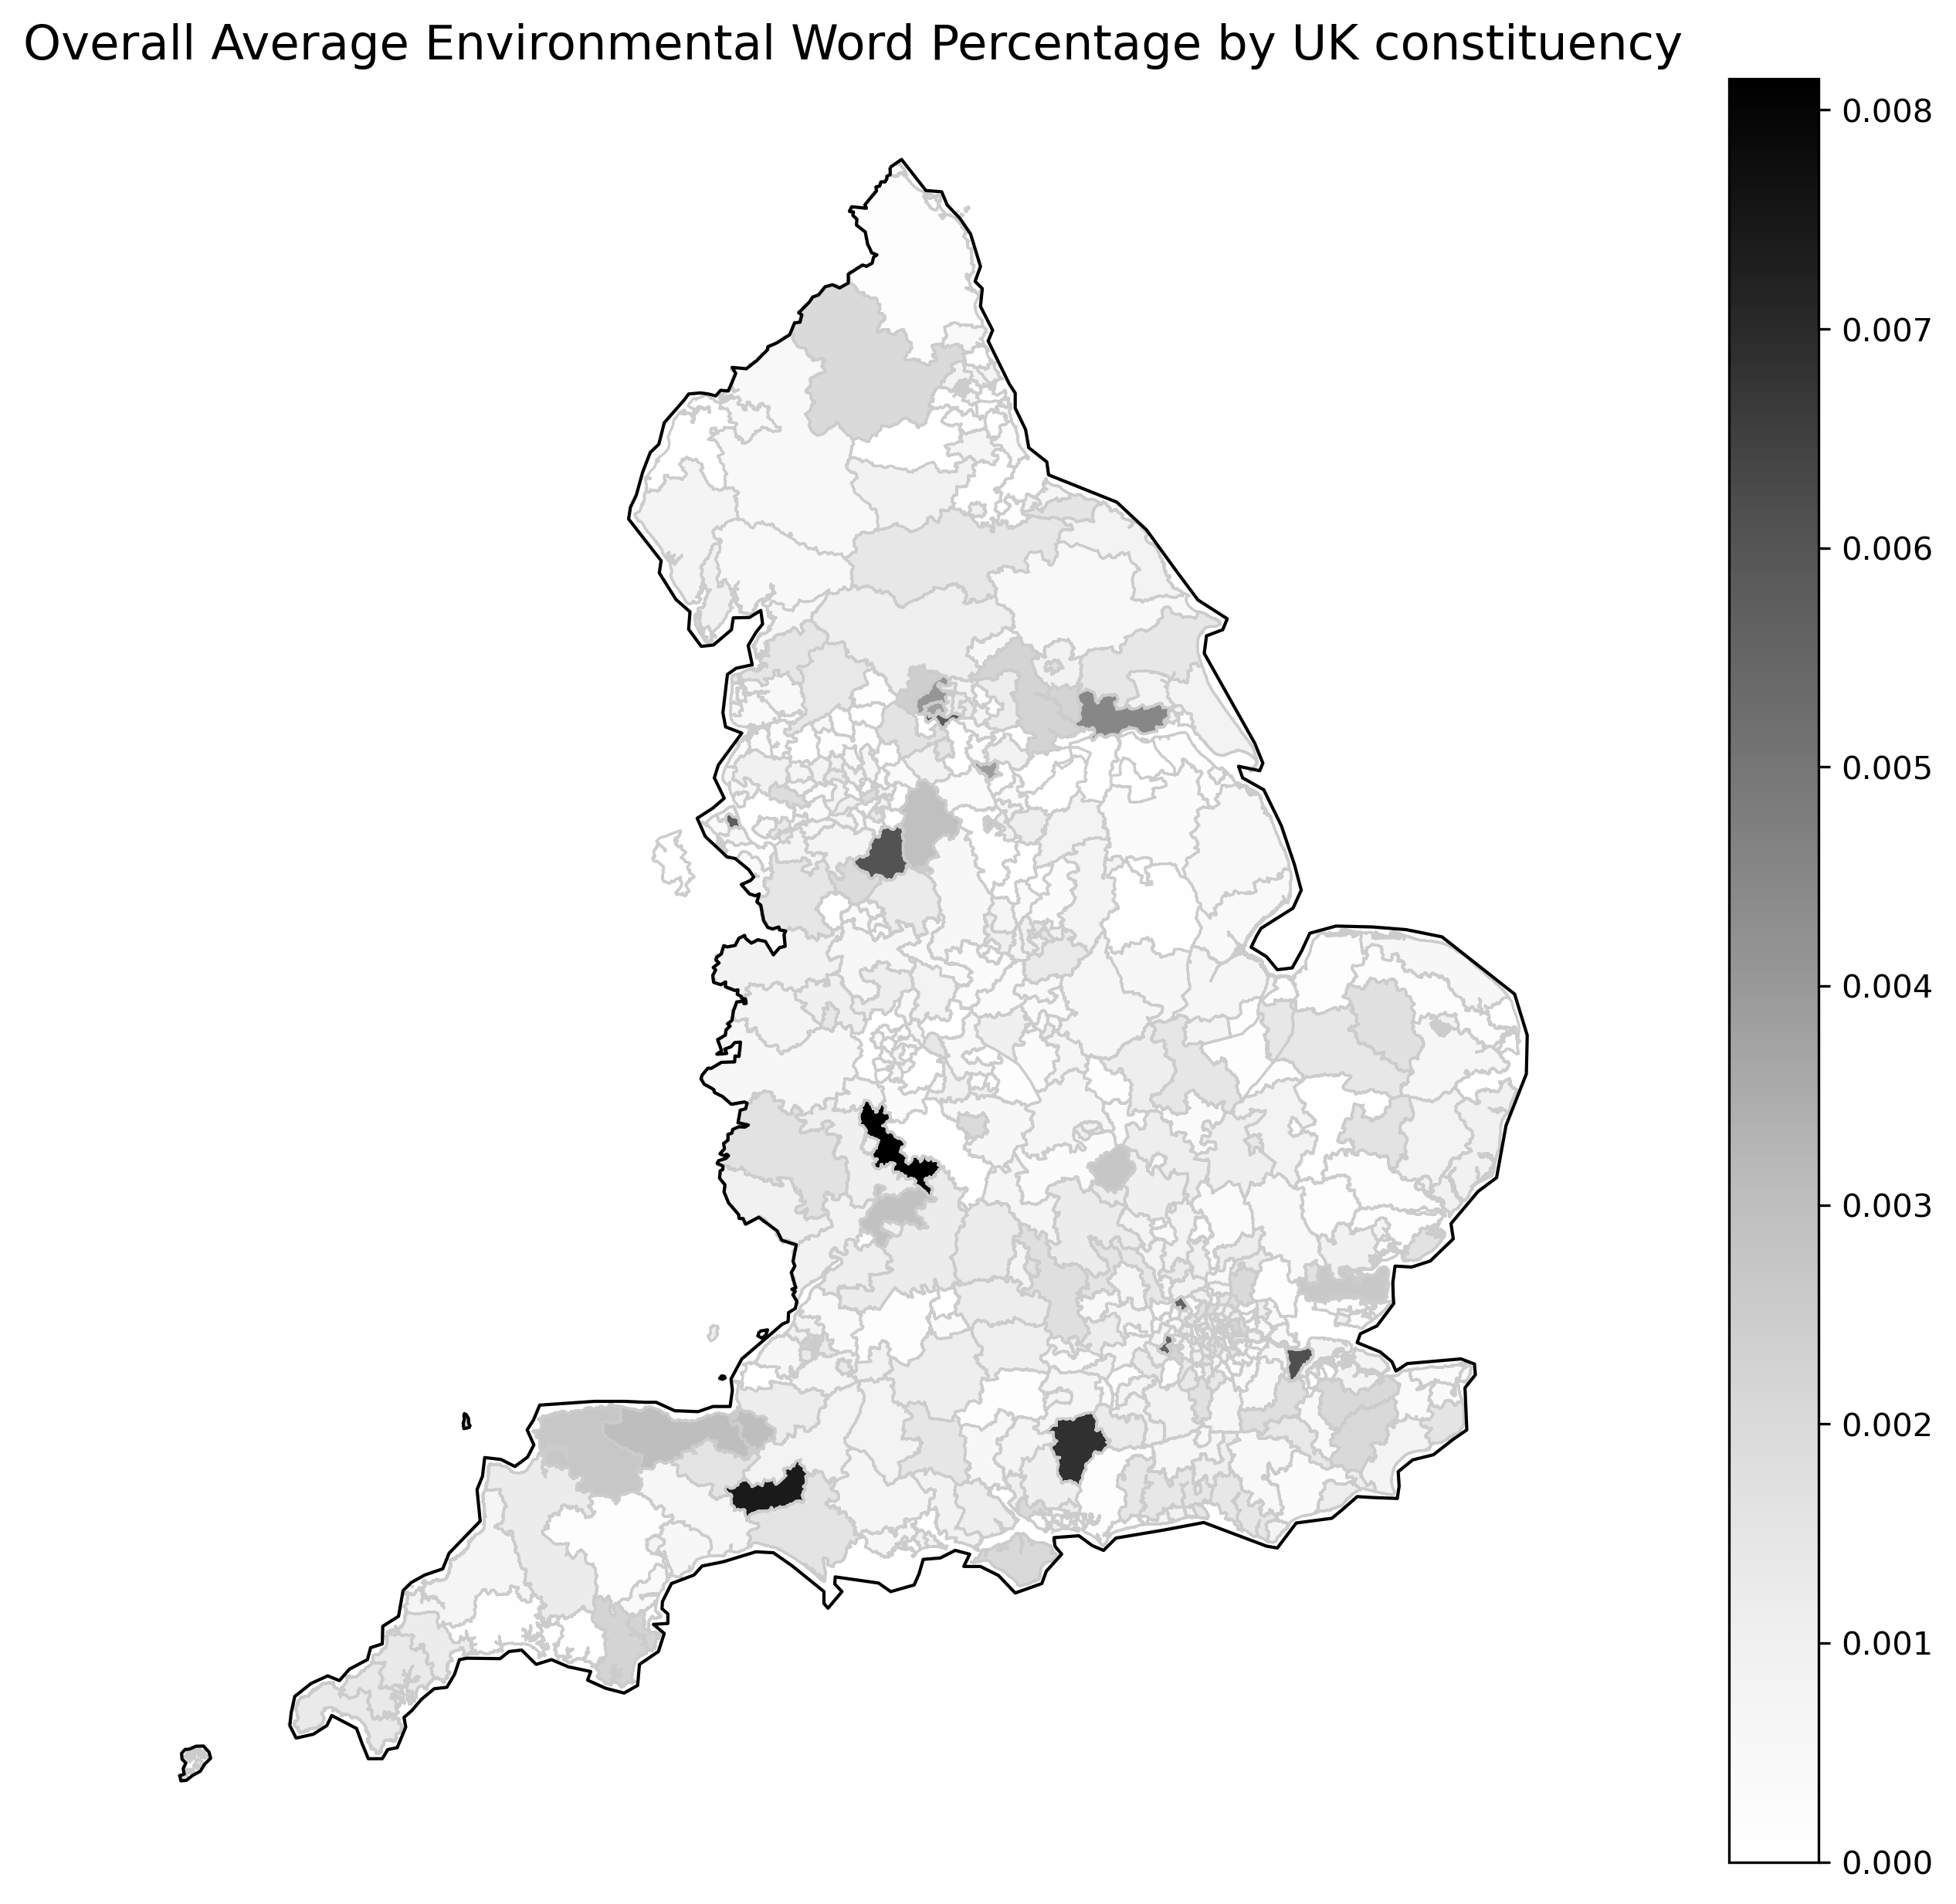
\includegraphics[width=0.55\textwidth]{Figure_1.png}
	\caption{Mean Environmental Mentions By Constituency}
	\label{fig:meanenvbycon}
\end{wrapfigure}




The overall distribution of environmental words used in campaign leaflets across England regardless of political party or election year is shown in Figure~\ref{fig:meanenvbycon} This groups the environmental mentions by constituency and then takes the mean of the percentage of environmental words out of total words for each of the constituencies. From this range of this figure, it is clear that most consituencies have a relatively low mean of environmental mentions, with the highest mean being 0.008\% of total words in the leaflet, with many constituencies having very close to an average of 0\% of environmental words mentioned. This very low number, especially when compared to the overall number of words in each leaflet, which can range from 100 to 1000 words. This suggests that environmental issues are not a primary focus in most constituencies, regardless of political party or election year. However, this figure provides preliminary evidence that the variation across consituencies is a non-zero value.


\begin{figure}[htbp]
    \centering
    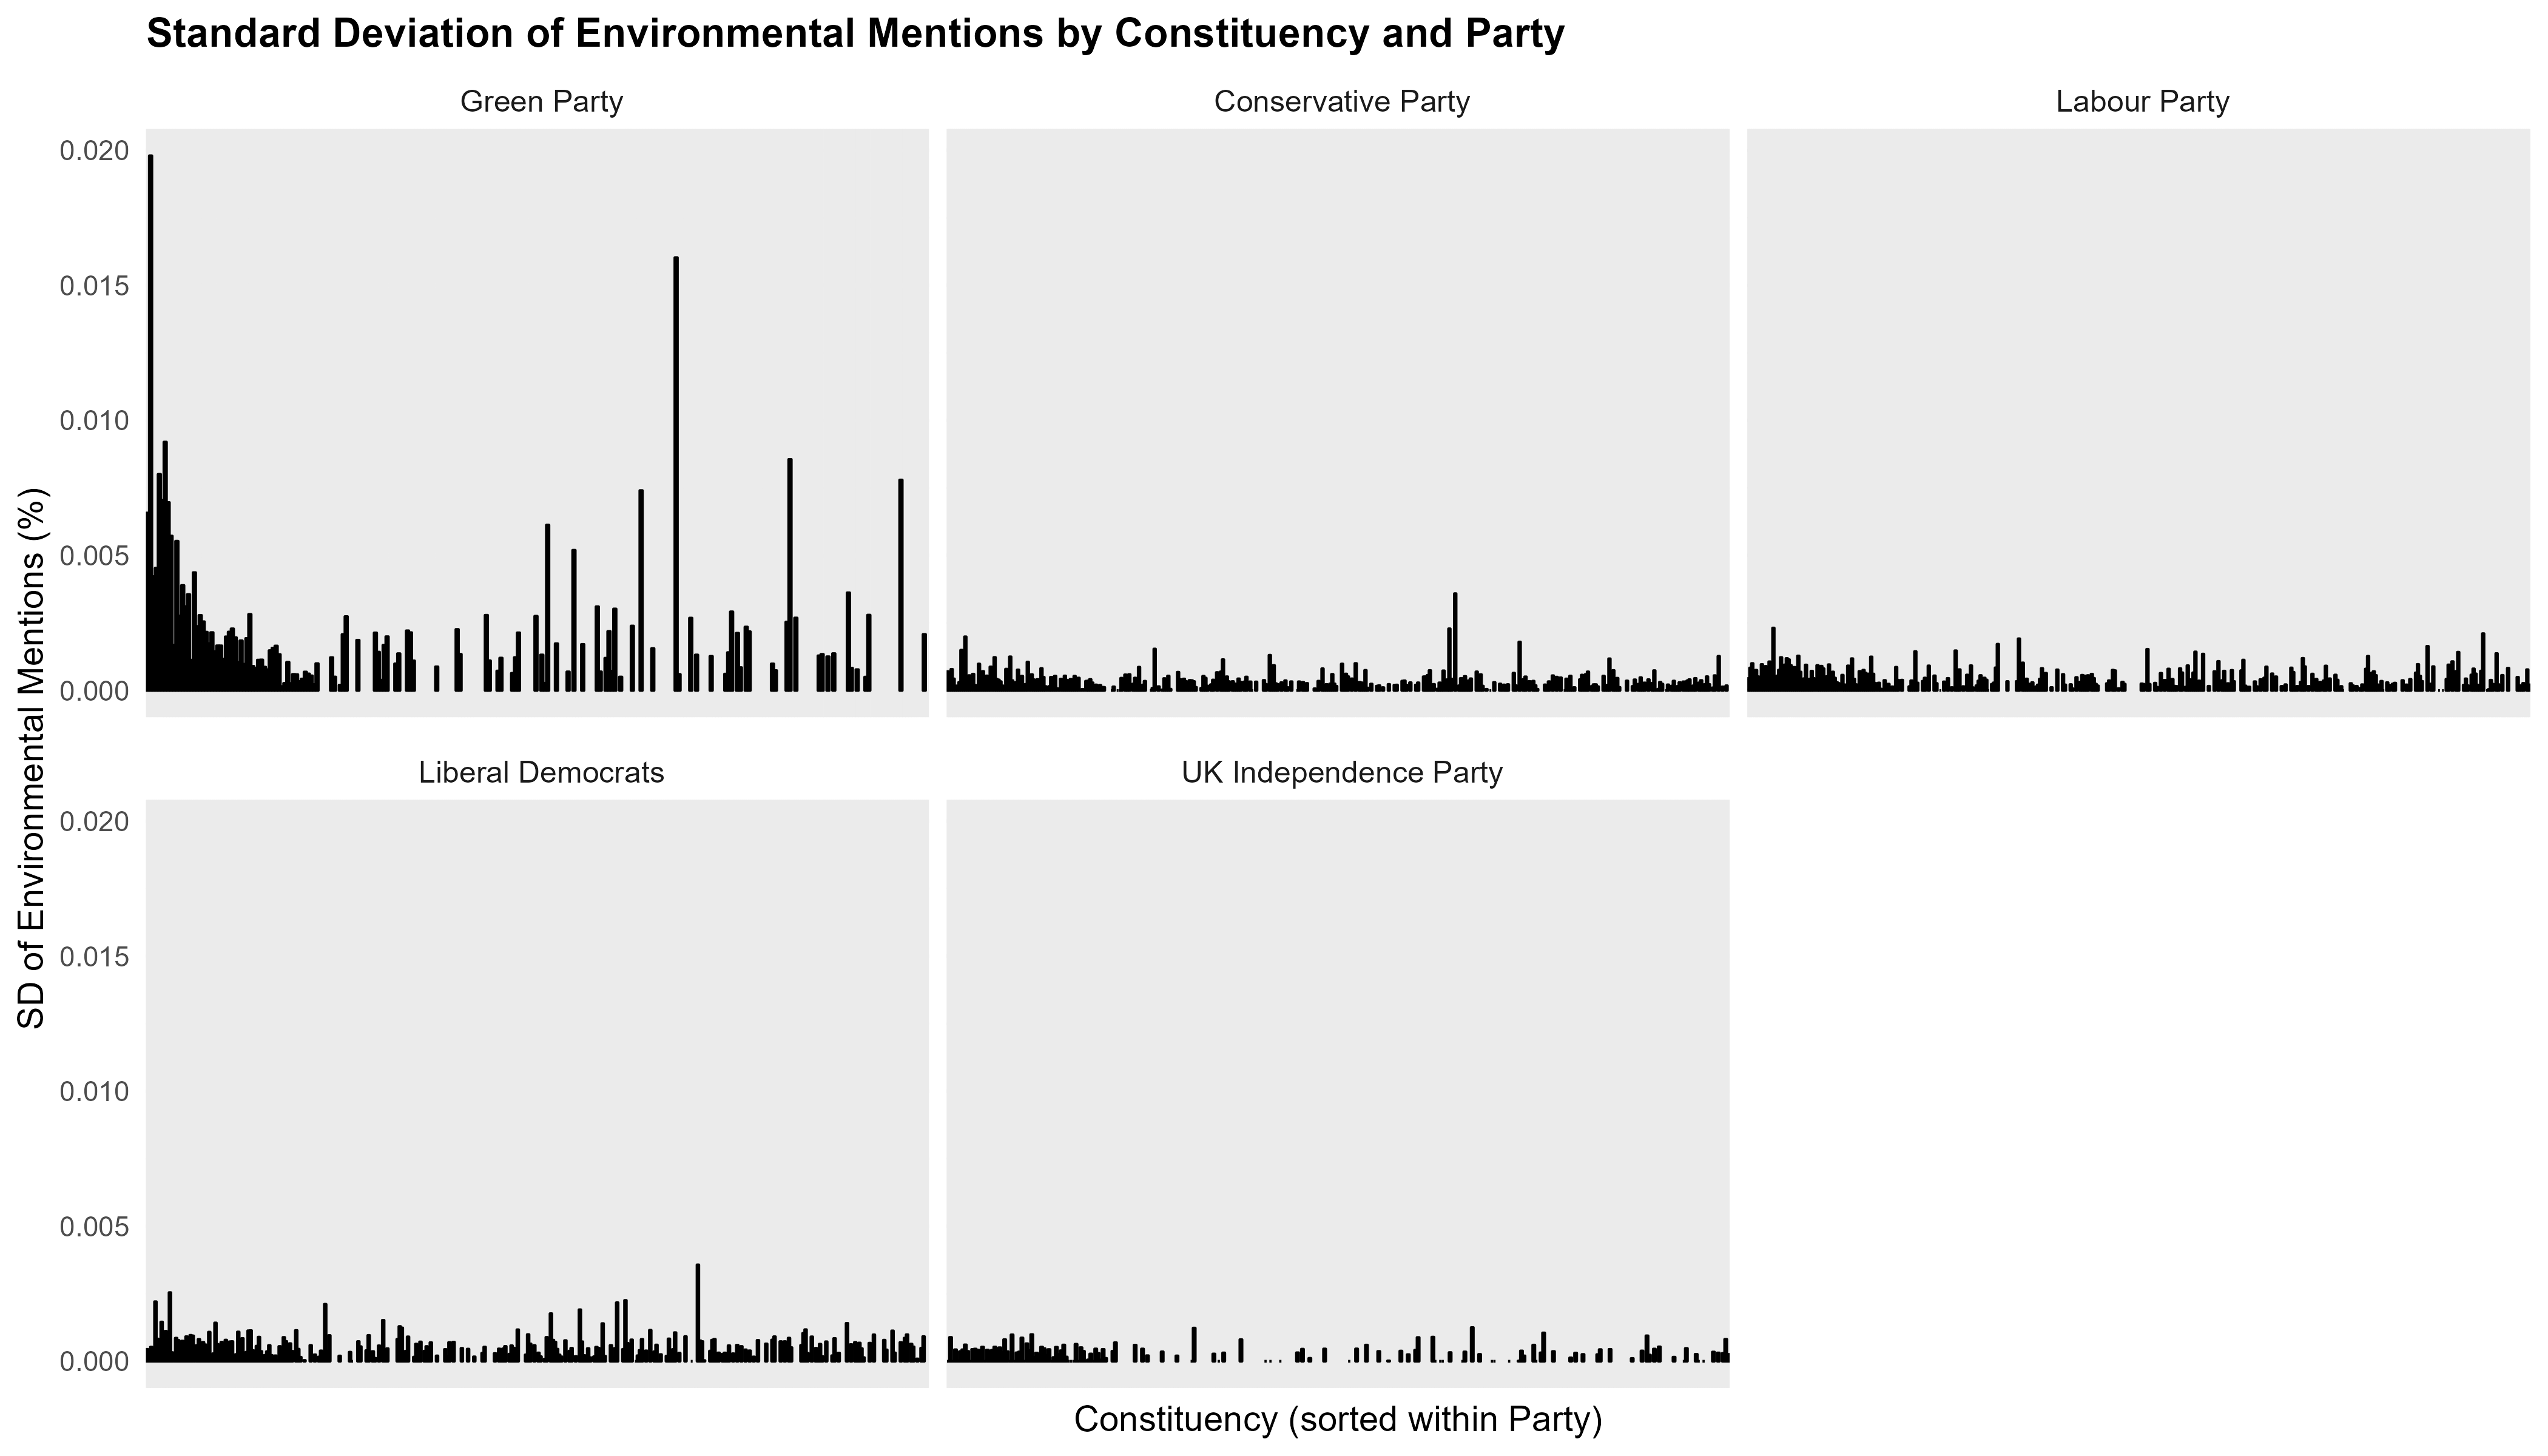
\includegraphics[width=\textwidth, height=0.9\textheight, keepaspectratio]{Figure_2.png}
    \caption{Standard Deviation Breakdown By Party}
    \label{fig:sd_party_const}
\end{figure}


\begin{figure}[htbp]
    \centering
    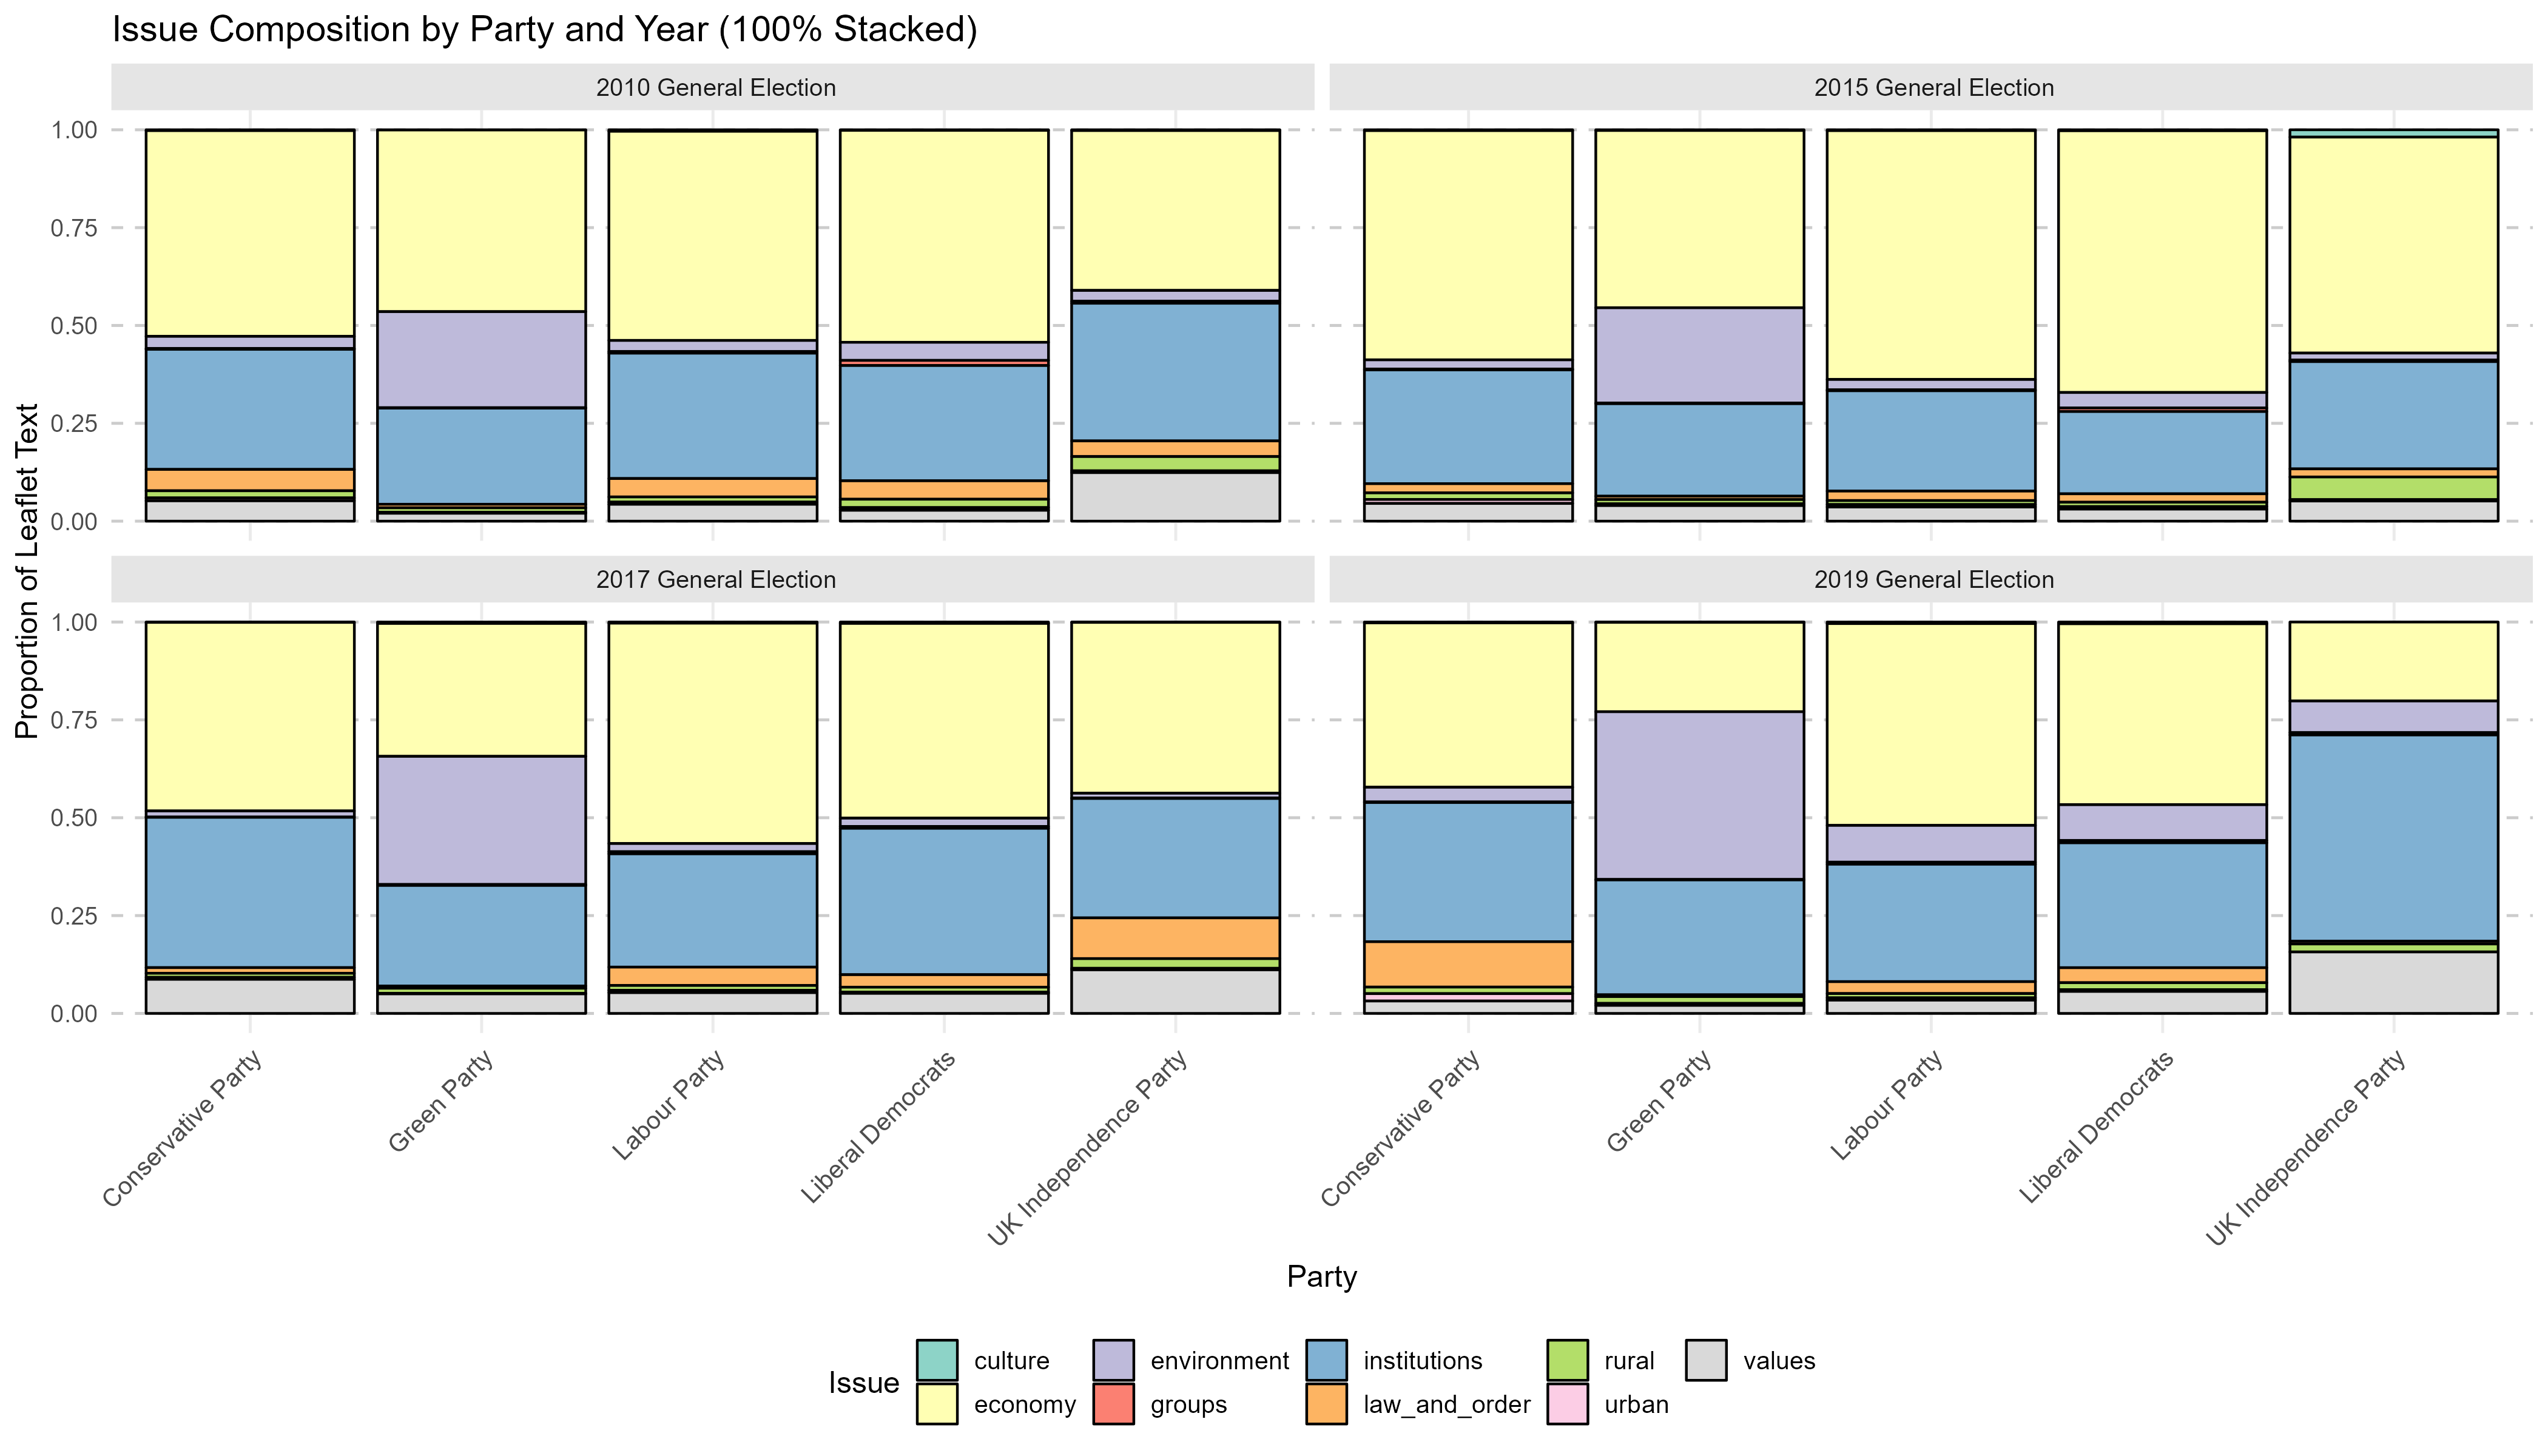
\includegraphics[width=\textwidth, height=0.9\textheight, keepaspectratio]{Figure_3.png}
    \caption{Stacked Topic Mentions by Year and Party}
    \label{fig:stacked_year_party}
\end{figure}

To further demonstrate that there is significant variation within environmental discussion in constituencies within the same political party, Figure~\ref{fig:sd_party_const} represents the standard deviation of each constituency from the mean environmental mention percentage. As demonstrated in the figure, the Green Party has the highest standard deviation, indicating that there is a large variation in environmental mentions across constituencies within the Green Party. This suggests that while the Green Party may have a higher overall percentage of environmental mentions, there is still significant variation in how much each constituency focuses on environmental issues. The other parties show more moderate variation, while still demonstrating that the mentions are not uniform across constituencies in the same party.





As the overall percentage of environmental mentions by constituency is quite low, a potentially more useful descriptor of what is happening in each election broadly is the breakdown of the percentages of each political topic by year and political party. Figure~\ref{fig:stacked_year_party} shows a stacked breakdown of the percentage of each political topic by year and party. As demonstrated, regardless of election year, the Green Party has the highest percentage of environmental mentions compared to the other parties, while also showing a significant focus on the economy as well as institutions. In contrast, the other parties all demonstrate a focus more significantly on both the economy and institutions, with less focus on all other political topics. This is in line with what would be expected that the Green Party has the highest mentions, with each other political party shower greater dedication to other political topics.


%also double check all the numbers in the tables, make sure they are correct and that the stars are in the right place



% Table 1: Simple OLS Regression Results
\begin{table}[!htbp] \centering
	\caption{Simple OLS Regression Results for Environmental Mention Percentage}
	\label{tab:OLS}
	\footnotesize % Make all text smaller
	\setlength{\tabcolsep}{4pt} % Reduce column spacing
	\renewcommand{\arraystretch}{0.9} % Reduce row spacing
\begin{tabular}{@{\extracolsep{5pt}}lc}
\\[-1.8ex]\hline
\hline \\[-1.8ex]
 & \multicolumn{1}{c}{\textit{Dependent variable:}} \\
 & \multicolumn{1}{c}{\textit{Environmental Mention Percentage}} \\
\cline{2-2}
\\[-1.8ex] & \textasciitilde . \\
\hline \\[-1.8ex]
 Party Conservative Party & $-$0.005$^{***}$ \\ 
	& (0.0001) \\
 Party Labour Party & $-$0.005$^{***}$ \\
	& (0.0001) \\
 Party Liberal Democrats & $-$0.005$^{***}$ \\
	& (0.0001) \\ 
 Party UK Independence Party & $-$0.005$^{***}$ \\
	& (0.0001) \\
 2015 Election & $-$0.0001$^{**}$ \\
	& (0.0001) \\
 2017 Election & $-$0.00004 \\
	& (0.0001) \\
 2019 Election & 0.001$^{***}$ \\
	& (0.0001) \\ 
 Median Age & $-$0.00001 \\
	& (0.00001) \\
 Rural Proportion & 0.00004 \\
	& (0.0001) \\
 Working Class Proportion & $-$0.001 \\
	& (0.001) \\
 Intermediate Proportion & 0.001 \\
	& (0.001) \\
 Professional Proportion & 0.001 \\
	& (0.001) \\
 Total Student Percentage & $-$0.001 \\
	& (0.001) \\
 Overall Weather Standard Deviation & 0.00001$^{**}$ \\ 
	& (0.00000) \\
 Liberal Democrat Share & 0.001$^{*}$ \\
	& (0.0003) \\
 Labour Party Share & 0.001$^{*}$ \\
	& (0.0003) \\
 Other Party Share & 0.001$^{*}$ \\
	& (0.0003) \\
 Conservative Party Share & 0.001$^{*}$ \\
	& (0.0003) \\
 Constant & $-$0.052$^{*}$ \\
	& (0.031) \\ 
\hline \\[-1.8ex]
Observations & 3,904 \\
R$^{2}$ & 0.625 \\
Adjusted R$^{2}$ & 0.623 \\
Residual Std. Error & 0.001 (df = 3885) \\
F Statistic & 359.861$^{***}$ (df = 18; 3885) \\
\hline 
\hline \\[-1.8ex]
\textit{Note:}  & \multicolumn{1}{r}{$^{*}$p$<$0.1; $^{**}$p$<$0.05; $^{***}$p$<$0.01} \\
\end{tabular}
\end{table}





% Table created by stargazer v.5.2.3 by Marek Hlavac, Social Policy Institute. E-mail: marek.hlavac at gmail.com
% Date and time: Wed, Jun 04, 2025 - 18:10:28
\begin{table}[!htbp] \centering
	\caption{Fixed Effects Models for Each Party with Election-Year Controls}
	\label{tab:party_fixed_effects}
	\scriptsize % Make text smaller
	\setlength{\tabcolsep}{6pt} % Adjust column spacing
	\renewcommand{\arraystretch}{1.2} % Increase row spacing
\begin{tabular}{@{\extracolsep{6pt}}lccccc}
\\[-1.8ex]\hline
\hline \\[-1.8ex]
 & \multicolumn{5}{c}{\textit{Dependent variable: Mean Environmental Mentions}} \\
\cline{2-6} 
\\[-1.8ex] & Green Party & Conservative & Labour & Lib Dems & UKIP \\      
\\[-1.8ex] & (1) & (2) & (3) & (4) & (5)\\
\hline \\[-1.8ex]
Median Age & $-$0.0001 & 0.00001 & $-$0.00000 & $-$0.00002 & $-$0.00000 \\ 
	& (0.0001) & (0.00001) & (0.00001) & (0.00001) & (0.00001) \\
Rural Population & 0.001 & $-$0.0001 & 0.0001 & 0.0001 & $-$0.0001 \\
	& (0.002) & (0.0001) & (0.0002) & (0.0002) & (0.0002) \\
Working Class & $-$0.009 & $-$0.002 & 0.001 & 0.006$^{**}$ & 0.001 \\
	& (0.021) & (0.002) & (0.002) & (0.003) & (0.002) \\ 
Intermediate Class & 0.007 & $-$0.004$^{*}$ & 0.001 & 0.004 & 0.004 \\
	& (0.021) & (0.002) & (0.002) & (0.003) & (0.003) \\
Professional Class & $-$0.017 & 0.002 & 0.002 & 0.008$^{***}$ & 0.002 \\ 
	& (0.021) & (0.002) & (0.002) & (0.003) & (0.002) \\
Student Count & $-$0.008 & $-$0.002 & 0.004$^{**}$ & 0.002 & 0.001 \\
	& (0.015) & (0.001) & (0.002) & (0.002) & (0.002) \\
Weather Variance & 0.0001 & $-$0.00000 & $-$0.00001 & 0.00002$^{*}$ & 0.00004$^{***}$ \\ 
	& (0.0001) & (0.00000) & (0.00001) & (0.00001) & (0.00001) \\
Labour Share & 0.00002 & $-$0.00000 & $-$0.00000 & $-$0.00001$^{*}$ & 0.00000 \\ 
	& (0.00003) & (0.00000) & (0.00000) & (0.00000) & (0.00000) \\
Lib Dem Share & $-$0.0004 & 0.0005 & 0.0003 & 0.001 & $-$0.001 \\
	& (0.005) & (0.0004) & (0.001) & (0.001) & (0.001) \\
Other Share & $-$0.0001$^{*}$ & $-$0.00001 & $-$0.00000 & 0.00000 & $-$0.00000 \\
	& (0.00004) & (0.00000) & (0.00000) & (0.00001) & (0.00000) \\ 
Conservative Share & 0.00000 & $-$0.00000 & 0.00001$^{**}$ & 0.00000 & $-$0.00000 \\
	& (0.00004) & (0.00000) & (0.00000) & (0.00000) & (0.00000) \\
 \hline \\[-1.8ex]
Observations & 387 & 1,025 & 1,116 & 1,023 & 377 \\ 
R$^{2}$ & 0.078 & 0.028 & 0.068 & 0.042 & 0.142 \\
Adjusted R$^{2}$ & $-$1.212 & $-$0.971 & $-$0.701 & $-$1.062 & $-$1.734 \\
\hline
\hline \\[-1.8ex]
\textit{Note:}  & \multicolumn{5}{r}{$^{*}$p$<$0.1; $^{**}$p$<$0.05; $^{***}$p$<$0.01} \\
\end{tabular}
\end{table} 



\subsection{Model 1: OLS Regression}



Table~\ref{tab:OLS} shows the results of a simple OLS regression model, which includes environmental mention percentages as the dependent variable with political party dummy variables with the Green Party as a reference category, election dummy variables with the 2010 Election as the reference category, median age, rural and urban population, profession categories, student percentage, weather standard deviation, and past vote share as independent variables. The model has an R-squared value of 0.625, indicating that approximately 62.5\% of the variance in environmental mention percentages can be explained by the independent variables included in the model.

The results show that the Conservative Party (\(\beta = -0.005, p < 0.001\)), Labour Party (\(\beta = -0.005, p < 0.001\)), Liberal Democrats (\(\beta = -0.005, p < 0.001\)), and UK Independence Party (\(\beta = -0.005, p < 0.001\)) all have a significant negative relationship with environmental mention percentages. This suggests that, holding all other factors constant, a leaflet from the Green Party is more likely to include a higher percentage of environmentally focused words, providing evidence for \textbf{\hyperlink{H3}{H3}}. The 2015 election also has a significant negative relationship with environmental mention percentages (\(\beta = -0.0001, p < 0.05\)), while the 2019 election has a significant positive relationship (\(\beta = 0.001, p < 0.001\)), indicating that leaflets from the 2019 election had, on average, higher environmental mention percentages across all constituencies compared to the 2010 Election, while the 2015 election contained significantly less mentions compared to the 2010 election.

Furthermore, the median age, rural proportion, working class proportion, intermediate proportion, professional proportion, and total student percentage do not have significant relationships with environmental mention percentages. This suggests that these demographic factors do not significantly impact the frequency of environmental mentions in campaign leaflets, providing evidence against \textbf{\hyperlink{H1}{H1}} and \textbf{\hyperlink{H2}{H2}}.

What appears to be significantly related to environmental mentions, however, is the overall weather standard deviation (\(\beta = 0.00001, p < 0.05\)), indicating that constituencies with greater weather variability are more likely to have higher environmental mention percentages in their campaign leaflets. This suggests that constituencies that experience more weather extremes may encourage local campaigners to discuss the environment and climate issues in their campaign leaflets, providing evidence for \textbf{\hyperlink{H5}{H5}}.

Lastly, this model indicates that the past vote share in a constituency does have a significant positive relationship with environmental mention percentages, such that local campaigners are more likely to mention the environment as the vote share of any political party increases (\(\beta = 0.001, p < 0.1\)). This effect, however, may be better examined in, as it is unclear how this mechanism may function within specific parties and the competition they face.


\subsection{Model 2: Fixed Effects Models for Each Party with Election-Year Controls}

This second model, although showing negative adjusted R-squared values, demonstrates that each party is sensitive to constituency-level factors that may not impact the campaign strategies of the other competition parties. For example, in the Green Party model, the only significant factor is that of the share of 'other' parties (not Labour, Conservative, or Liberal Democrats) in a constituency, which has a negative relationship with environmental mention percentages (\(\beta = -0.0001, p < 0.1\)). This suggests that constituencies with a higher share of 'other' parties are less likely to have high environmental mention percentages in their campaign leaflets.

In regard to \textbf{\hyperlink{H4}{H4}}, the results indicate that the past vote share of the Conservative Party has a significant effect only on the Labour Party, with every one unit increase in vote share for the Conservative Party being associated with a 0.00001 unit increase in environmental mention percentages (\(\beta = 0.00001, p < 0.05\)) in Labour Party leaflets. The Labour Party also has a significant positive relationship with the share of students in a constituency (\(\beta = 0.004, p < 0.05\)), indicating that constituencies with a higher proportion of students are more likely to have higher environmental mention percentages in Labour Party campaign leaflets.

The Conservative Party appears to be unaffected by past vote share of any party, with the only factor significantly associated to environmental mentions being the proportion of individuals in the Intermediate Class (\(\beta = -0.004, p < 0.1\)). The Liberal Democrat Party also shows a significant positve relationship between both the proportion of individuals in the Professional Class as well as in the Working Class (\(\beta = 0.008, p < 0.001\) and \(\beta = 0.006, p < 0.05\), respectively), indicating that constituencies with a higher proportion of individuals in these classes are more likely to have higher environmental mention percentages. 

The Liberal Democrat party also shows a relationship between weather variance and environmental mentions (\(\beta = 0.00002, p < 0.1\)), as well as a significant positive relationship with the share of Labour Party votes in a constituency (\(\beta = 0.001, p < 0.05\)). The UK Independence party seems to only show a significant relationship between weather variance and environmental mentions (\(\beta = 0.00004, p < 0.001\)), indicating that constituencies with greater weather variability are more likely to have higher environmental mention percentages in UK Independence Party campaign leaflets.



\section{Discussion}


The time period analysed in this project provides an interesting and complicated political atmosphere to navigate. In the 2010 election, the earliest election analysed in this study, political geography and marginality of constituencies mattered greatly in campaigning \citep{johnstonLearningElectoralGeography2013}. However, Brexit referendum in 2016, there was a shift towards two-party politics in England in the 2017 election \citep{hoboltBrexit2017UK2018,prosserStrangeDeathMultiparty2018}, as voters who may have previously voted for the UK Independence shifted loyalty to the Conservative Party and Remain voters were more inclined to vote for the Labour Party. This trend was continued in 2019, which saw greater efficacy on the part of Conservatives at unifying Leave voters, giving the party an advantage over the Labour party who struggled to unify voters in this way \citep{cuttsBrexit2019General2020}. However, the 2017 election showed Labour's changing demographic of supporters, as those that are younger and in more diverse areas demonstrated more inclination to vote for Labour \citep{heath2017GeneralElection2017}. The complexitiy in the political climate during this time period, although perhaps too complex to fully address in this study, provides a rich context for the preliminary research of quantifying environmental mentions and attempting to understanding the underlying mechanisms behind these mentions.

Table~\ref{tab:OLS} was used with both political party and election year included as dummy variables. This approach allowed for more flexible modelling of year-specific effects without imposing the assumption that temporal differences are constant across all units, as fixed effects do. This allows for a broader understanding of how each of the included factors may impact environmental mentions in campaign leaflets. An interesting finding in this model was that the 2015 and 2019 Elections were the only elections to have results that indicate that the election year itself had a significant impact on environmental mentions compared to the 2010 Election, with the 2015 Election having a negative relationship and the 2019 Election having a positive relationship with environmental mentions. This may indicate that the 2017 Election was unique following the Brexit referendum, returning to a focus on political geography and marginality of constituencies in campaigning \citep{johnstonLearningElectoralGeography2013}. Further analysis with the inclusion of specific factors for each election year may prove to be a fruitful avenue for future research.

This model also shows unexpected results in regard to the impact that vote share has on the presence of environmental mentions in campaign leaflets. While it was hypothesised that higher vote share in previous elections for the Conservative party would be associated with lower environmental mentions in campaign leaflets, the results of the model show that a higher vote share for all parties has a positive relationship with environmental mentions in campaign leaflets. While the OLS model is useful in demonstrating that vote share was a useful inclusion in the model, this result perhaps indicates that the results would be better understood when looking at the campaigns of each political party individually.

Table~\ref{tab:party_fixed_effects} highlights two important points: there is evidence that local campaigns differ from one another even when they are from the same political party, and that campaign strategies are sensitive to different constituency-level factors that may not impact the campaign strategies of other parties. This marks the first step understanding the specific magnitude that each of these factors has on environmental mentions in campaign leaflets, as well as it may guide future research with this dataset in discovering which factors have the most impact on campaigns and therefore are best able to enact political and social change.

An interesting observation in this model is that the Conservative Party seems to be only impacted by the proportion of individuals in the Intermediate Class, and the Liberal Democrats appear to be impacted by both the Working Class and Professional Class. The Intermediate Class has a negative relationship with environmental mentions in Conservative Party leaflets, while the Working Class and Professional Class have positive relationships with environmental mentions within their specific political party campaigns. This is unexpected, considering income is usually positively associated with environmental concern \citep{liu2024personal}. One possible explanation for this unexpected result is that the Working Class is comprised of a large number of individuals who may perhaps vary in occupation, interests, etc. \citep{le2008class}.

Furthermore, this model shows that the only variable that was significant in the same direction for more than one model is that of overall weather variance, with a positive effect for both Liberal Democrats and the UK Independence Party \((\beta = 0.00002, p < 0.1\), \(\beta = 0.00004, p < 0.001\)).

\subsection{Limitations}



This study, being the first report to use this specific dataset with a quantitative measure of political topic mentions, has several limitations that would be useful avenues for future research. First, this study condensed all forms of environmental mentions into one overarching category where all words regarding the environment or climate were treated the same. In other words, a political campaign could be negatively discussing the environment and other parties that may be focused on it, and this would be treated the same as a leaflet that is writing about the environment from a place of climate and environmental concern. This limits the scope and full understanding of how politicians discuss the environment. Future research could perform an analysis of each subcategory of environmental issues to see where and why variation occurs across parties and constituencies, as well as to run a sentiment analysis on the text to determine if the mentions are primarily positive or negative.

Another limitation arising from the structure of the dataset is that the vote share data used in this study does not include the Green Party, as they were not a significant party until 2015. This means that the vote share data for the 'Other' category includes both the Green Party and any other smaller parties that may have been present in a constituency. This could have had an impact on the results, specifically in the analysis of the Green party itself, as it is unclear whether vote share for the 'Other' category is primarily from the Green Party or from other smaller parties, possibly skewing the results.

As this study focused primarily on text scraping and analysis methods of election leaflet images, there are many avenues for future research that were not fully explored in this project. For instance, this project features several limitations in terms of how weather events affect various groups of people, specifically that weather data was used as opposed to natural disaster data in order for it to be converted to the constituency level in the analysis. Future research could also utilise media data to gain a fuller understanding of which communities are affected by climate change and natural disasteres, as suggested by \citet{siscoEffectsWeatherExperiences2021}. 


Lastly, as this project relied on data from many different sources and was converted to the constituency level regardless of its original form, a substantial amount of cases were lost for the final analysis. This is another limitation that should be addressed in future studies.
	


\section{Conclusion}

This study used novel methods to explore variations in campaign strategy across constituencies in England and created a new dataset that can be used for future work on any political topic, not just the environment. The results of this study highlight that, as would be expected, leaflets from the Green Party are more likely to include environmental mentions than leaflets from other parties. Furthermore, weather variability, social class, and vote share were all found to be significant predictors in at least one of the models shown. Urban and Rural Population did not appear to be significant in any of the models.

This project allows for large amounts of future research and highlights several issues with previous methods of analysis on political leaflets. The novel datasets that were created from this project can be used for further projects, as the complete scraped text is shown from all leaflets in the final dataset as well as the counts of words in each of the political speech categories. The methodology used to scrape text from the leaflets also appeared to perhaps introduce a new standard of analysis, since it was able to detect the same amount as human coders while also providing a quantitative measure to compare between quantity of text of various political topics. The scope of data available in this project due to the use of OCR methods introduce this method as one that could change the future of campaign research.

 


\bibliographystyle{elsarticle-harv}  % You can use 'elsarticle-num', 'elsarticle-harv', etc.

\bibliography{Dissertation2}  


\newpage








\section{Appendix}

\subsection{Data Collection and Processing Methods}

The outcome data was measured using leaflet data from OpenElections \citep{milazzo2020openelections}. This contained information from the 2010, 2015, 2017, and 2019 UK General Elections, with leaflets uploaded and coded based on constituency, party, issues mentioned, etc. The OpenElections data contained images of the leaflets as well as the metadata obtained by human coders. In order to enhance this dataset and separate it from other previously existing datasets, this study used text-scraping from image techniques. \citep{KerasocrKeras_ocrDocumentation,hoffstaetterPytesseractPythontesseractPython}. This process involved machine learning algorithms that detect text from an image and uses Optical Character Recognition (OCR) \citep{madhugiriExtractTextImages2022}. This was supplemented with Pytesseract's text orientation function that detects both the language of the text as well as if the text is rotated \citep{rosebrockCorrectingTextOrientation2022} in order to be able to flip the images that are rotated either 90 or 270 degrees. As there were over 18,000 images scraped from the OpenElections website, this step will be crucial in order to ensure that the highest possible amount of text is preserved. 



The text was then sorted using the Laver Garry dictionary \citep{laverEstimatingPolicyPositions2000} with frequencies of each category of words counted for each constituency, party, and year. The words pertaining to the environment from this dictionary are divided into pro-environment words (ie., "car", "chemical", "ecolog", "emission", "green", "planet", and "product") as well as con-environment words (ie., "product"). In addition to these words, I added a 'climate' subcategory consisting of the following words: "climate", "climate change", "global warming", "carbon emissions", and "greenhouse gases." These words were selected by reading through several leaflets and finding common words pertaining to the environment in order to best match the definition of environmentally related words to the human coders. Once the dictionary was used and the leaflets' text is divided into cleaned tokens, the environment (among the others) subcategories were condensed together and the number of words matching in any of the subcategories were counted and stored as a count variable in the dataset. This dataset therefore does not into account the type of environmental mentions included in the leaflets, although this could be an avenue for further research. 

Furthermore, as this study used text scraped from leaflets rather than articles or speeches, the pre-processing of the text followed a slightly different approach than standard text analysis projects. Rather than removing stop words and finding collocations, the data cleaning process  minimally processed the text data, primarily removing symbols and numbers. As the text was not necessarily in the correct order, this was necessary to make sure that the analysis doedids not miss any important mentions. The text data obtained from this process was then be compared back to the metadata that was created by human coders but was also used to examine issue salience and frequency of mentions beyond what can be done with human coders \citep{trummParliamentaryCandidatesTheir2023a}. The metadata for the leaflets only contained a binary measure of mentions: either the leaflet mentions the issue or it does not. Although this was useful for ensuring accuracy of the keras-OCR model, it does little in capturing a full image of fine details in campaigns. 
 


After the text was scraped, variation within each topic was measured between constituencies as well as between each party and election year. Data from Meteostat \citep{MeteostatPyPI} was used to collect weekly weather data from one year before the election date to the election date. This time period was chosen based on past literature suggesting that extreme weather events are most salient closer to the event \citep{viscontiEffectDifferentExtreme2024}.The data was then converted into a single variation variable, through taking the standard deviation of the aggregate weather data as a single measure of how inconsistent the weather is at each location and to measure any major changes that might be salient to those living there. This was to obtain a general summary of how weather patterns vary across the UK in the year leading up to each election.



\subsection{OCR Text-Scraping Accuracy}
The text scraping accuracy results for environmental mentions is shown in Table~ \ref{tab:envaccuracy}. The first accuracy score of 88.66\% means that for every time the metadata lists the environment as a mentioned issue, the OCR text-scraping methods also find at least 1 mention of an environmental-related word approximately 89\% of the time. This accuracy score, in the scope of this project, shows that the machine learning OCR method used to scrape the text, as well as the dictionary used, has an accuracy of almost 90\%. This is considerably good given the large volume of data and automated text-scraping methods on leaflets that vary in image quality.

The second accuracy score describes the frequency at which the metadata that was scraped from the OpenElections website lists the environment as one of the mentions during conditions in which the leaflet text that I scraped \textit{also} shows some mention of the environment. The score of 58.07\% indicates that, assuming my text-scraping methods are correct, the human coders only catch environmental mentions approximately 58.07\% of the time. 




\subsection{UKIP Example Images}


% Include the second image
\begin{figure}[H]
	\centering
	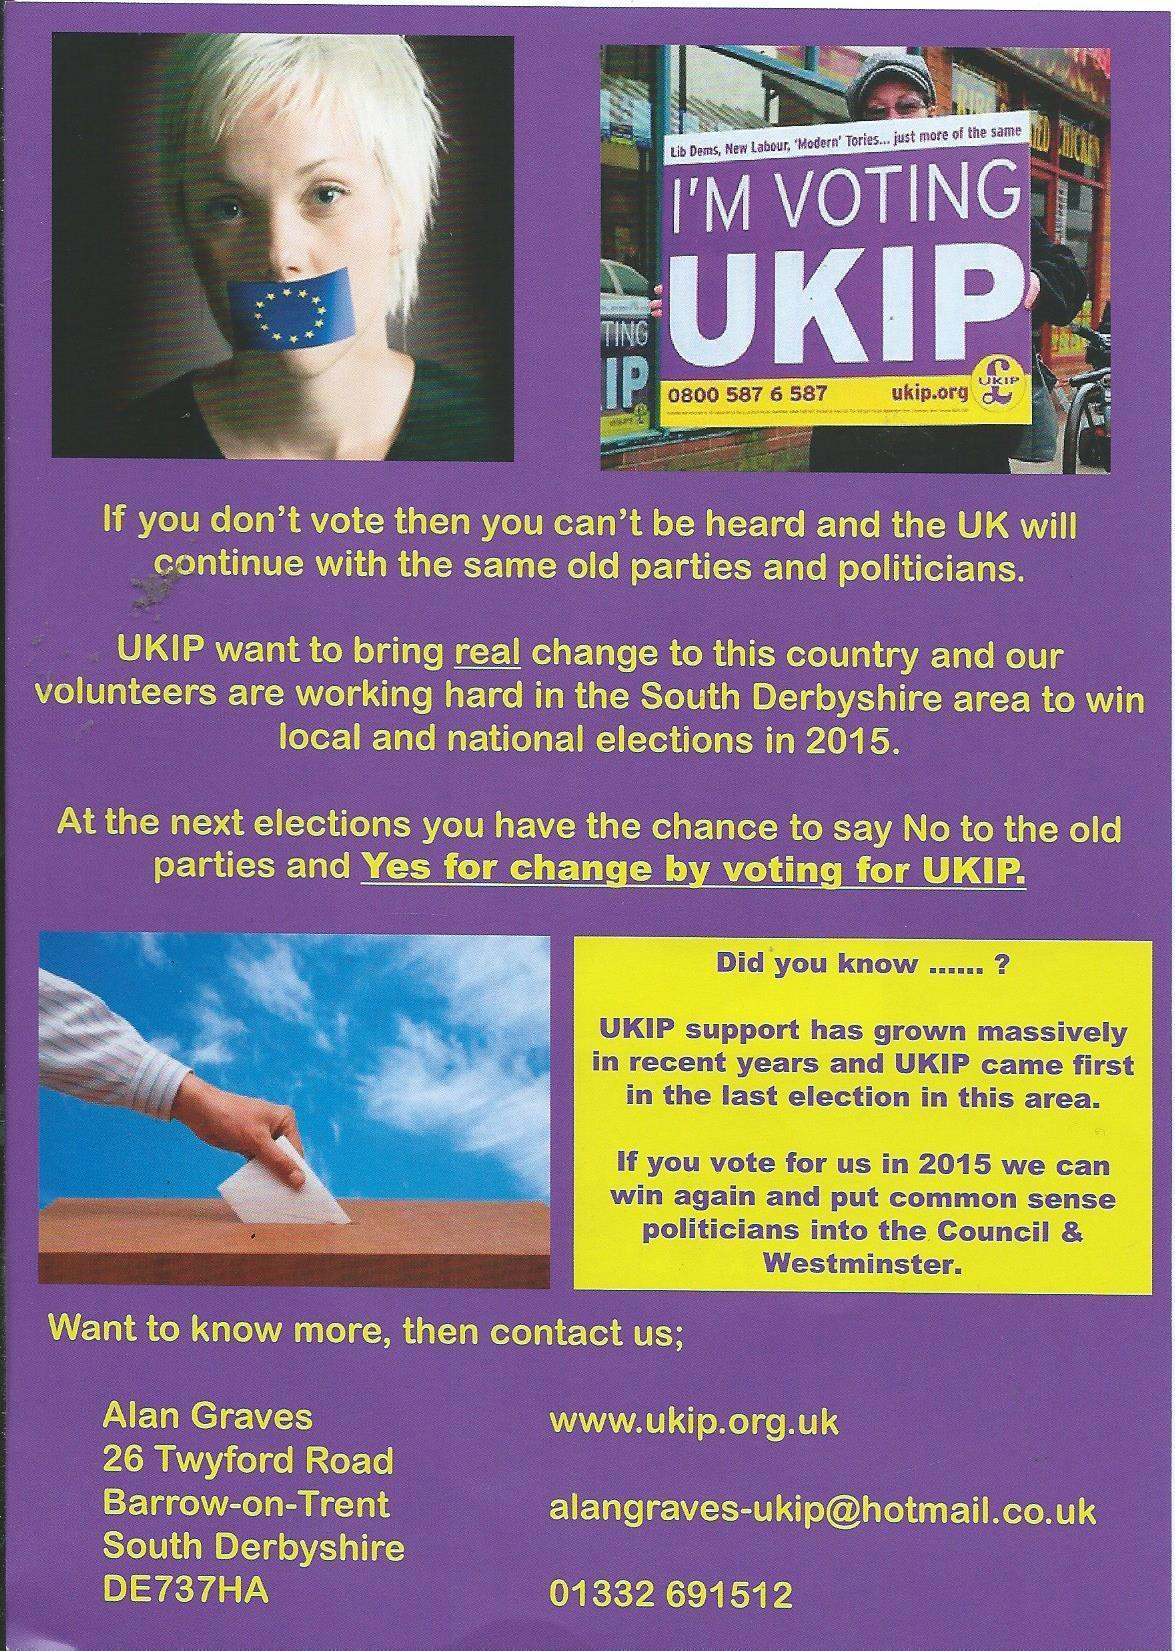
\includegraphics[width=0.3\textwidth]{Appendix_Figure_1.jpg}
	\caption{}
	\label{fig:Appendix_Figure_1}
\end{figure}

% Include the third image
\begin{figure}[H]
	\centering
	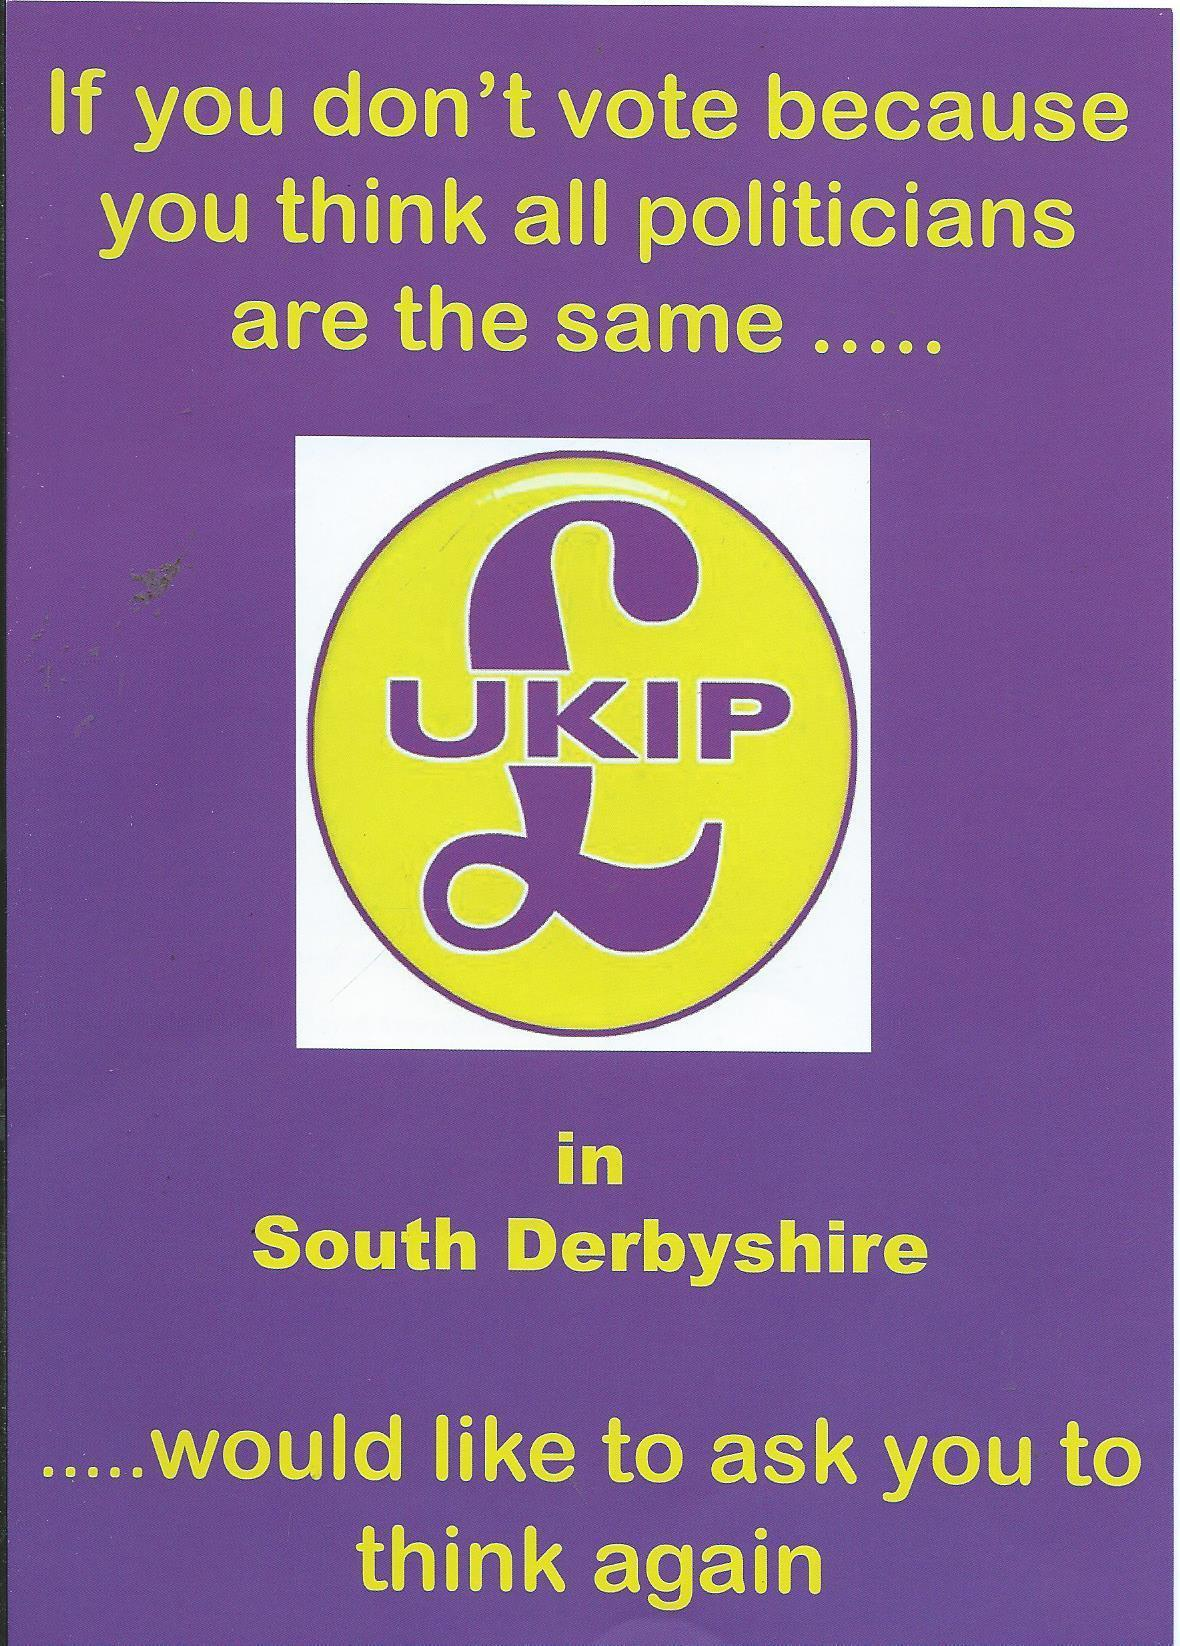
\includegraphics[width=0.3\textwidth]{Appendix_Figure_2.jpg}
	\caption{}
	\label{fig:Appendix_Figure_2}
\end{figure}

% Include the image without text wrapping
\begin{figure}[H]
	\centering
	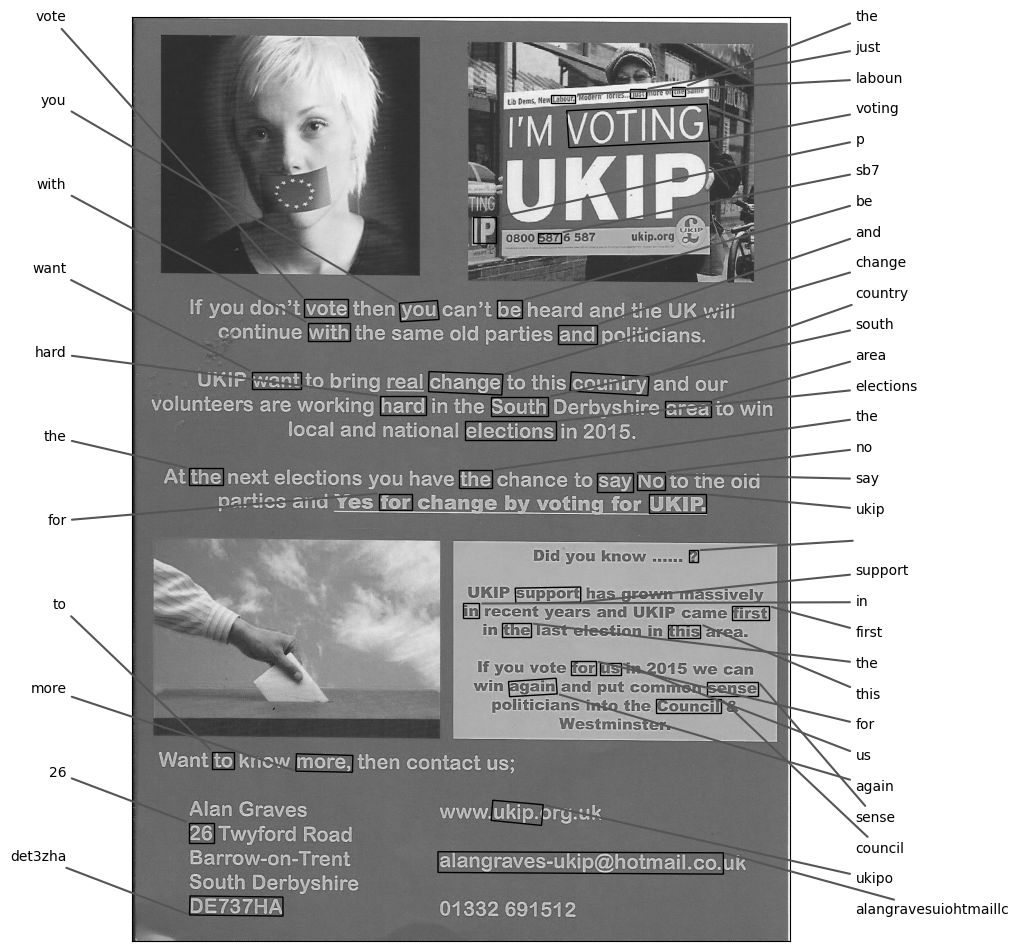
\includegraphics[width=0.58\textwidth]{Appendix_Figure_3.png}
	\caption{OCR Method on UKIP Example}
	\label{fig:ukip_example}
\end{figure}

\begin{table}[!htbp]  
	\centering
	\caption{Accuracy of Text-Scraping Methods on Environmental Issues} 
	\label{tab:envaccuracy} 
	\begin{tabular}{p{0.7\textwidth}cc}
			\hline
			Condition & Count & Accuracy \\ 
			\hline
			Accuracy of OCR detection when 'Environment' is in metadata & 2417/2726 & 88.66\% \\
			Accuracy of 'Environment' in metadata when OCR detects mentions & 2417/4162 & 58.07\% \\
			\hline
	\end{tabular}
\end{table}

\vspace{0.5cm}

As a robustness check to ensure that these results extend to the rest of the dataset, Table~\ref{tab:econaccuracy} displays the accuracy results for economy mentions as well. This table displays interesting results, such that the OCR methods used in tandem with the Laver Garry dictionary \citep{laverEstimatingPolicyPositions2000} to detect mentions of the economy are accurate in almost 100\% of the cases where the human-coded metadata shows an economic mention in the leaflet. 

Both Table~\ref{tab:econaccuracy} and Table~\ref{tab:envaccuracy} demonstrate a discrepancy in the human coded data versus the text scraped from the leaflet. It appears that in cases of both environmental and economic mentions that the OCR method detects more mentions of both topics. However, the accuracy score is quite high for detecting what has already been picked up by human coders. This would imply that the combination of the text scraping and the use of the Laver Garry dictionary is able to go beyond what is possible with human coders alone. Furthermore, this method could also be used in a further analysis to look at which words in each category specifically are used most frequently throughout the leaflets. 

\vspace{1cm}

\begin{table}[!htbp]
	\centering
	\caption{Accuracy of Text-Scraping Methods on Economic Issues}
	\label{tab:econaccuracy}
	\begin{tabular}{p{0.7\textwidth}cc}
			\hline
			Condition & Count & Accuracy \\
			\hline
			Accuracy of OCR detection when 'Economy' is in metadata & 5322/5373 & 99.05\% \\
			Accuracy of 'Economy' in metadata when OCR detects mentions & 5322/7073 & 75.24\% \\
			\hline
	\end{tabular}
\end{table}



\vspace{1cm}




One possible explanation for the variation between the accuracy levels regarding environmental mentions is that the human coders may have inconsistently labeled the leaflets as having environmental mentions when none are actually present. For instance, Figure~\ref{fig:ukip_example}\footnote{For readability, the entire OCR method was not included here, instead every fourth word detection is shown to demonstrate the effectiveness of the method. The entire unmarked leaflet is available in the appendix in Appendix Figure~\ref{fig:Appendix_Figure_1} and Figure~\ref{fig:Appendix_Figure_2}.} demonstrates a case where the metadata included the environment as a mentioned topic, but the OCR method does not detect any environmental mentions. Upon closer inspection, it appears that the OCR method performs accurately, as there are no discernible mentions of the environment in either of the images associated with that leaflet. This observation supports the robustness of the OCR text-scraping method and its suitability for subsequent analysis of variation in environmental mentions.

Additionally, it is unclear exactly how the human coders are deciding which categories are mentioned in the leaflets. The OpenElection website allows any site visitor to upload or code a leaflet based on mentions and issues in the images. This introduces a great amount of variation in how the leaflets are potentially classified, as individuals may vary in their knowledge of politics or individuals may not detect all of the issues on the leaflet. As the accuracy levels show that the OCR method detects a high proportion of what is found by human coders and, as shown in Figure~\ref{fig:ukip_example}, the metadata may not be entirely accurate, it seems as though the OCR method detects the same things that human coders would but goes beyond that to identify themes that require more political knowledge than the average person has.



\subsection{Leaflet Maps by Party}


\begin{figure}[htbp]  % Use [htbp] for figure placement
	\centering
	
	% Row 1
	\begin{minipage}[t]{0.335\textwidth}
		\centering
		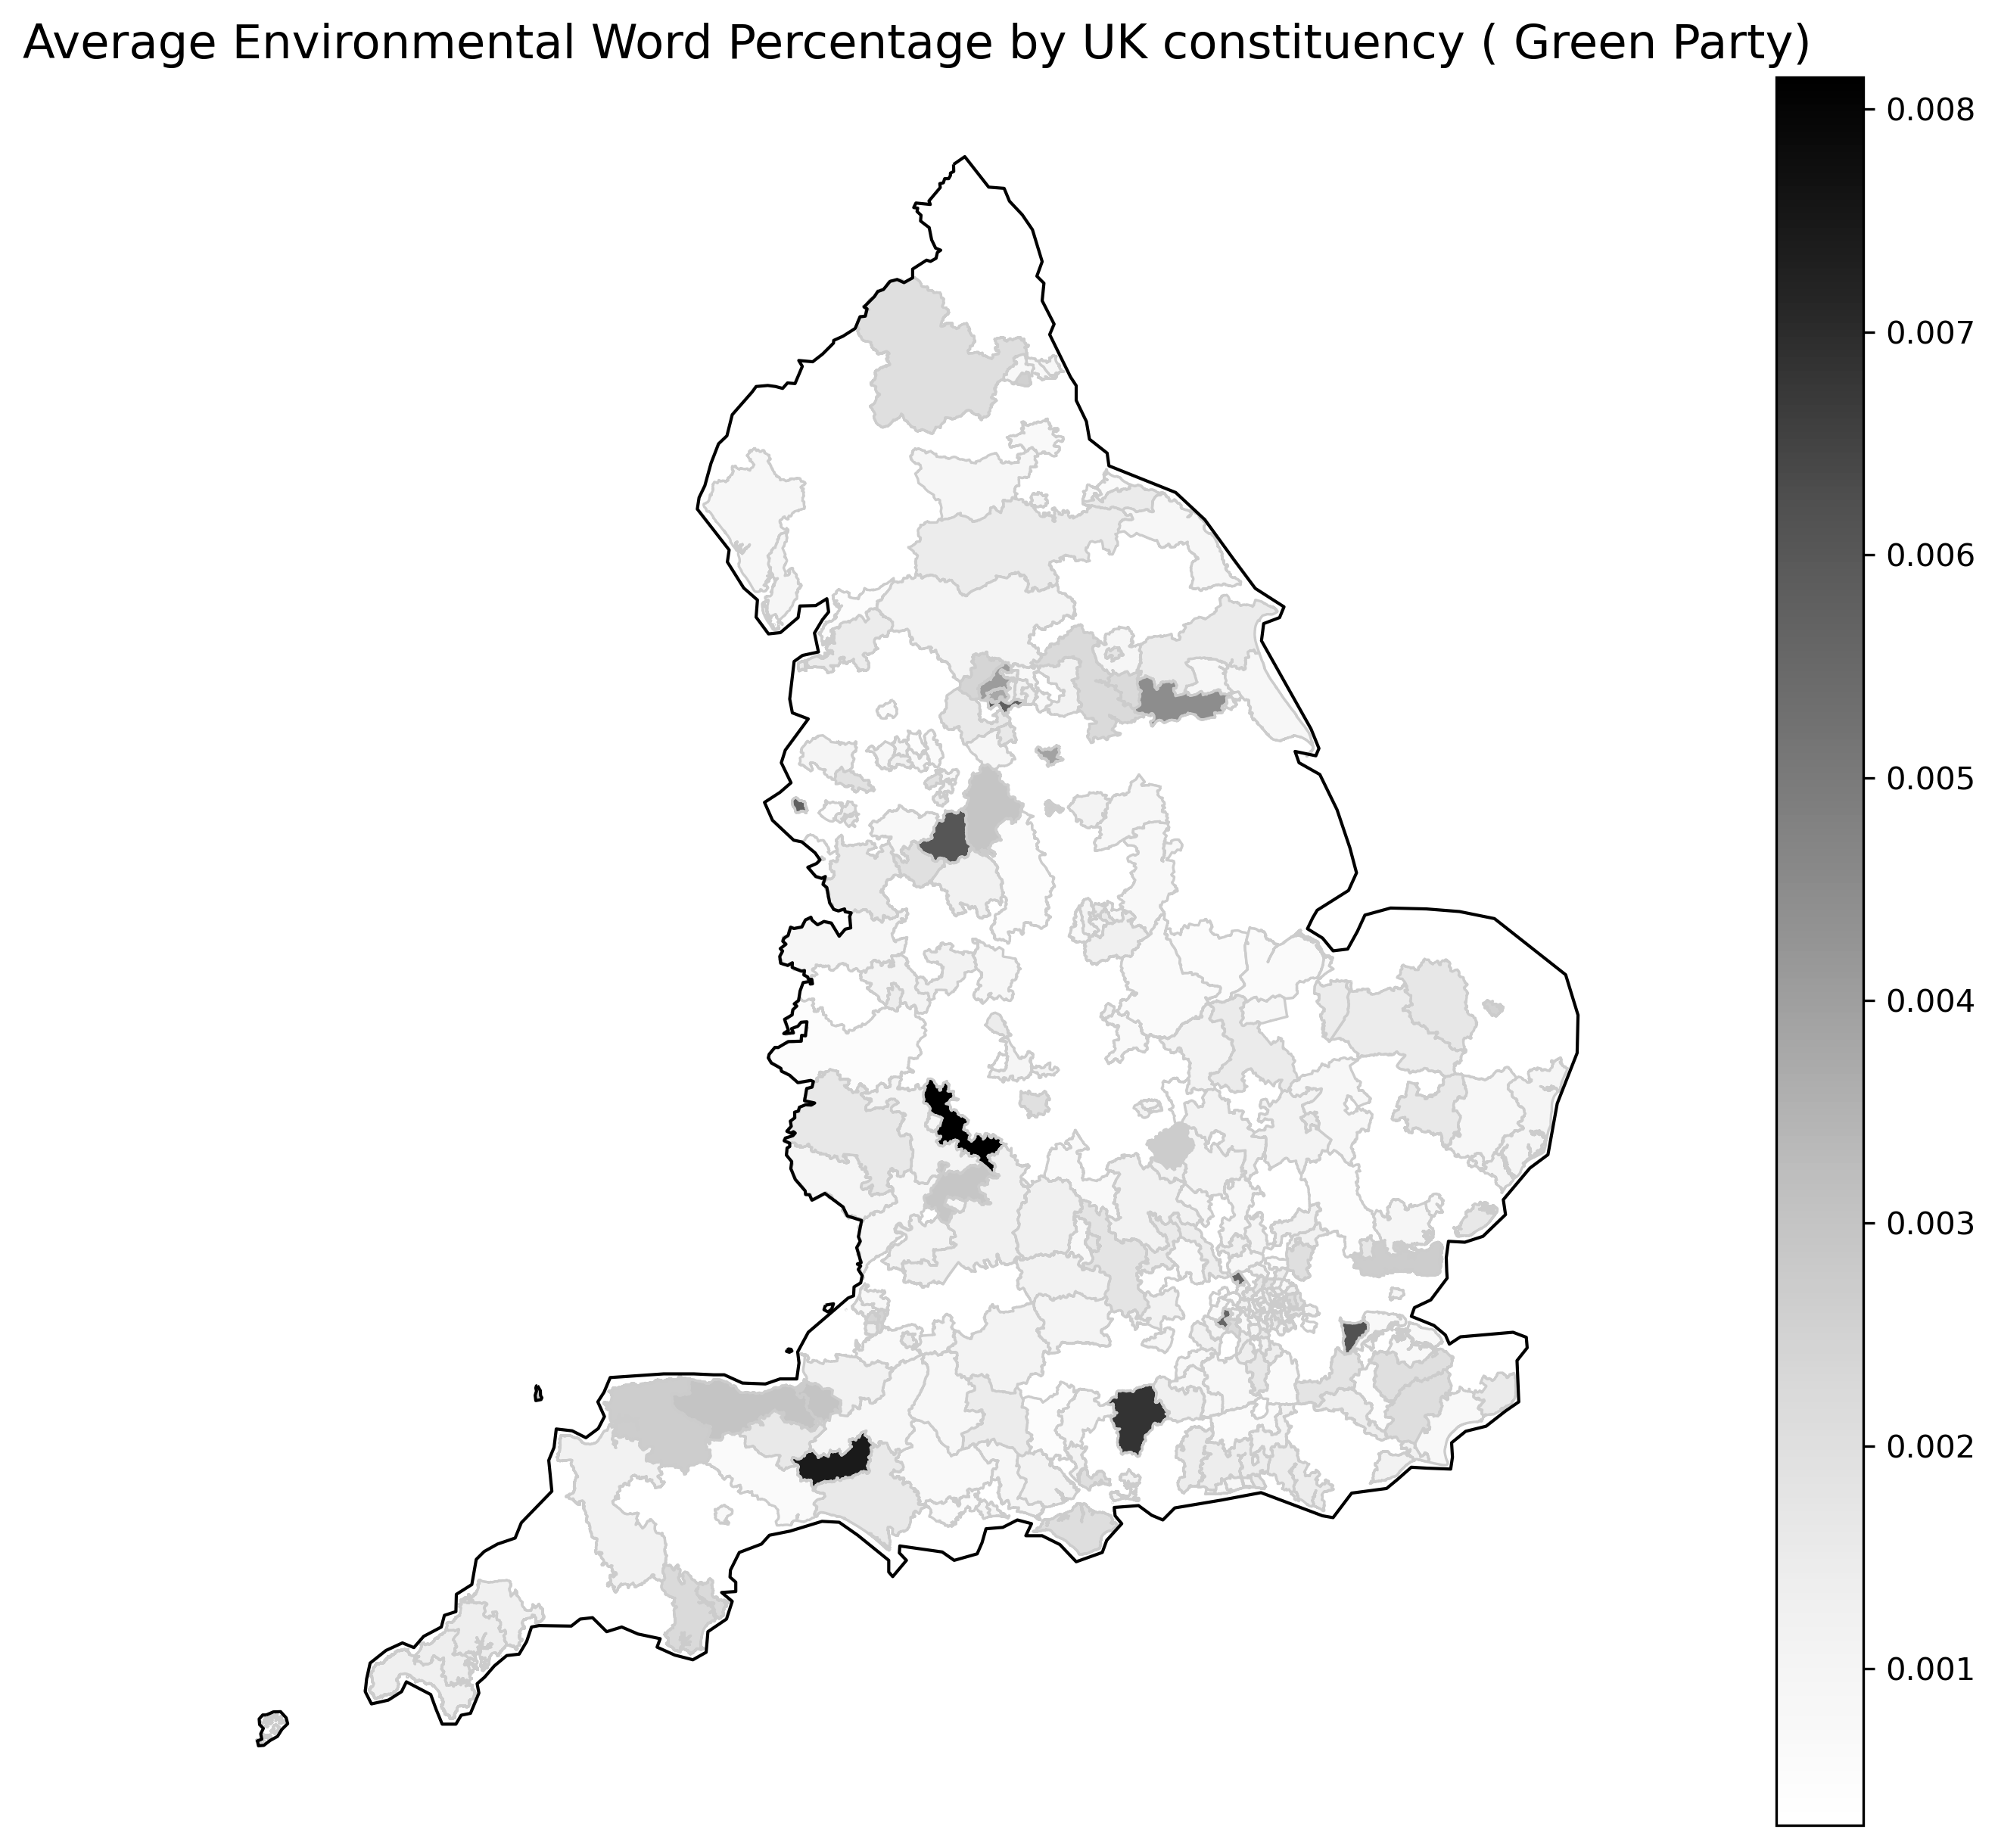
\includegraphics[width=\textwidth,height=0.68\textheight,keepaspectratio]{Appendix_Figure_4.png}
		\caption{Conservative Party}
	\end{minipage}\hfill
	\begin{minipage}[t]{0.335\textwidth}
		\centering
		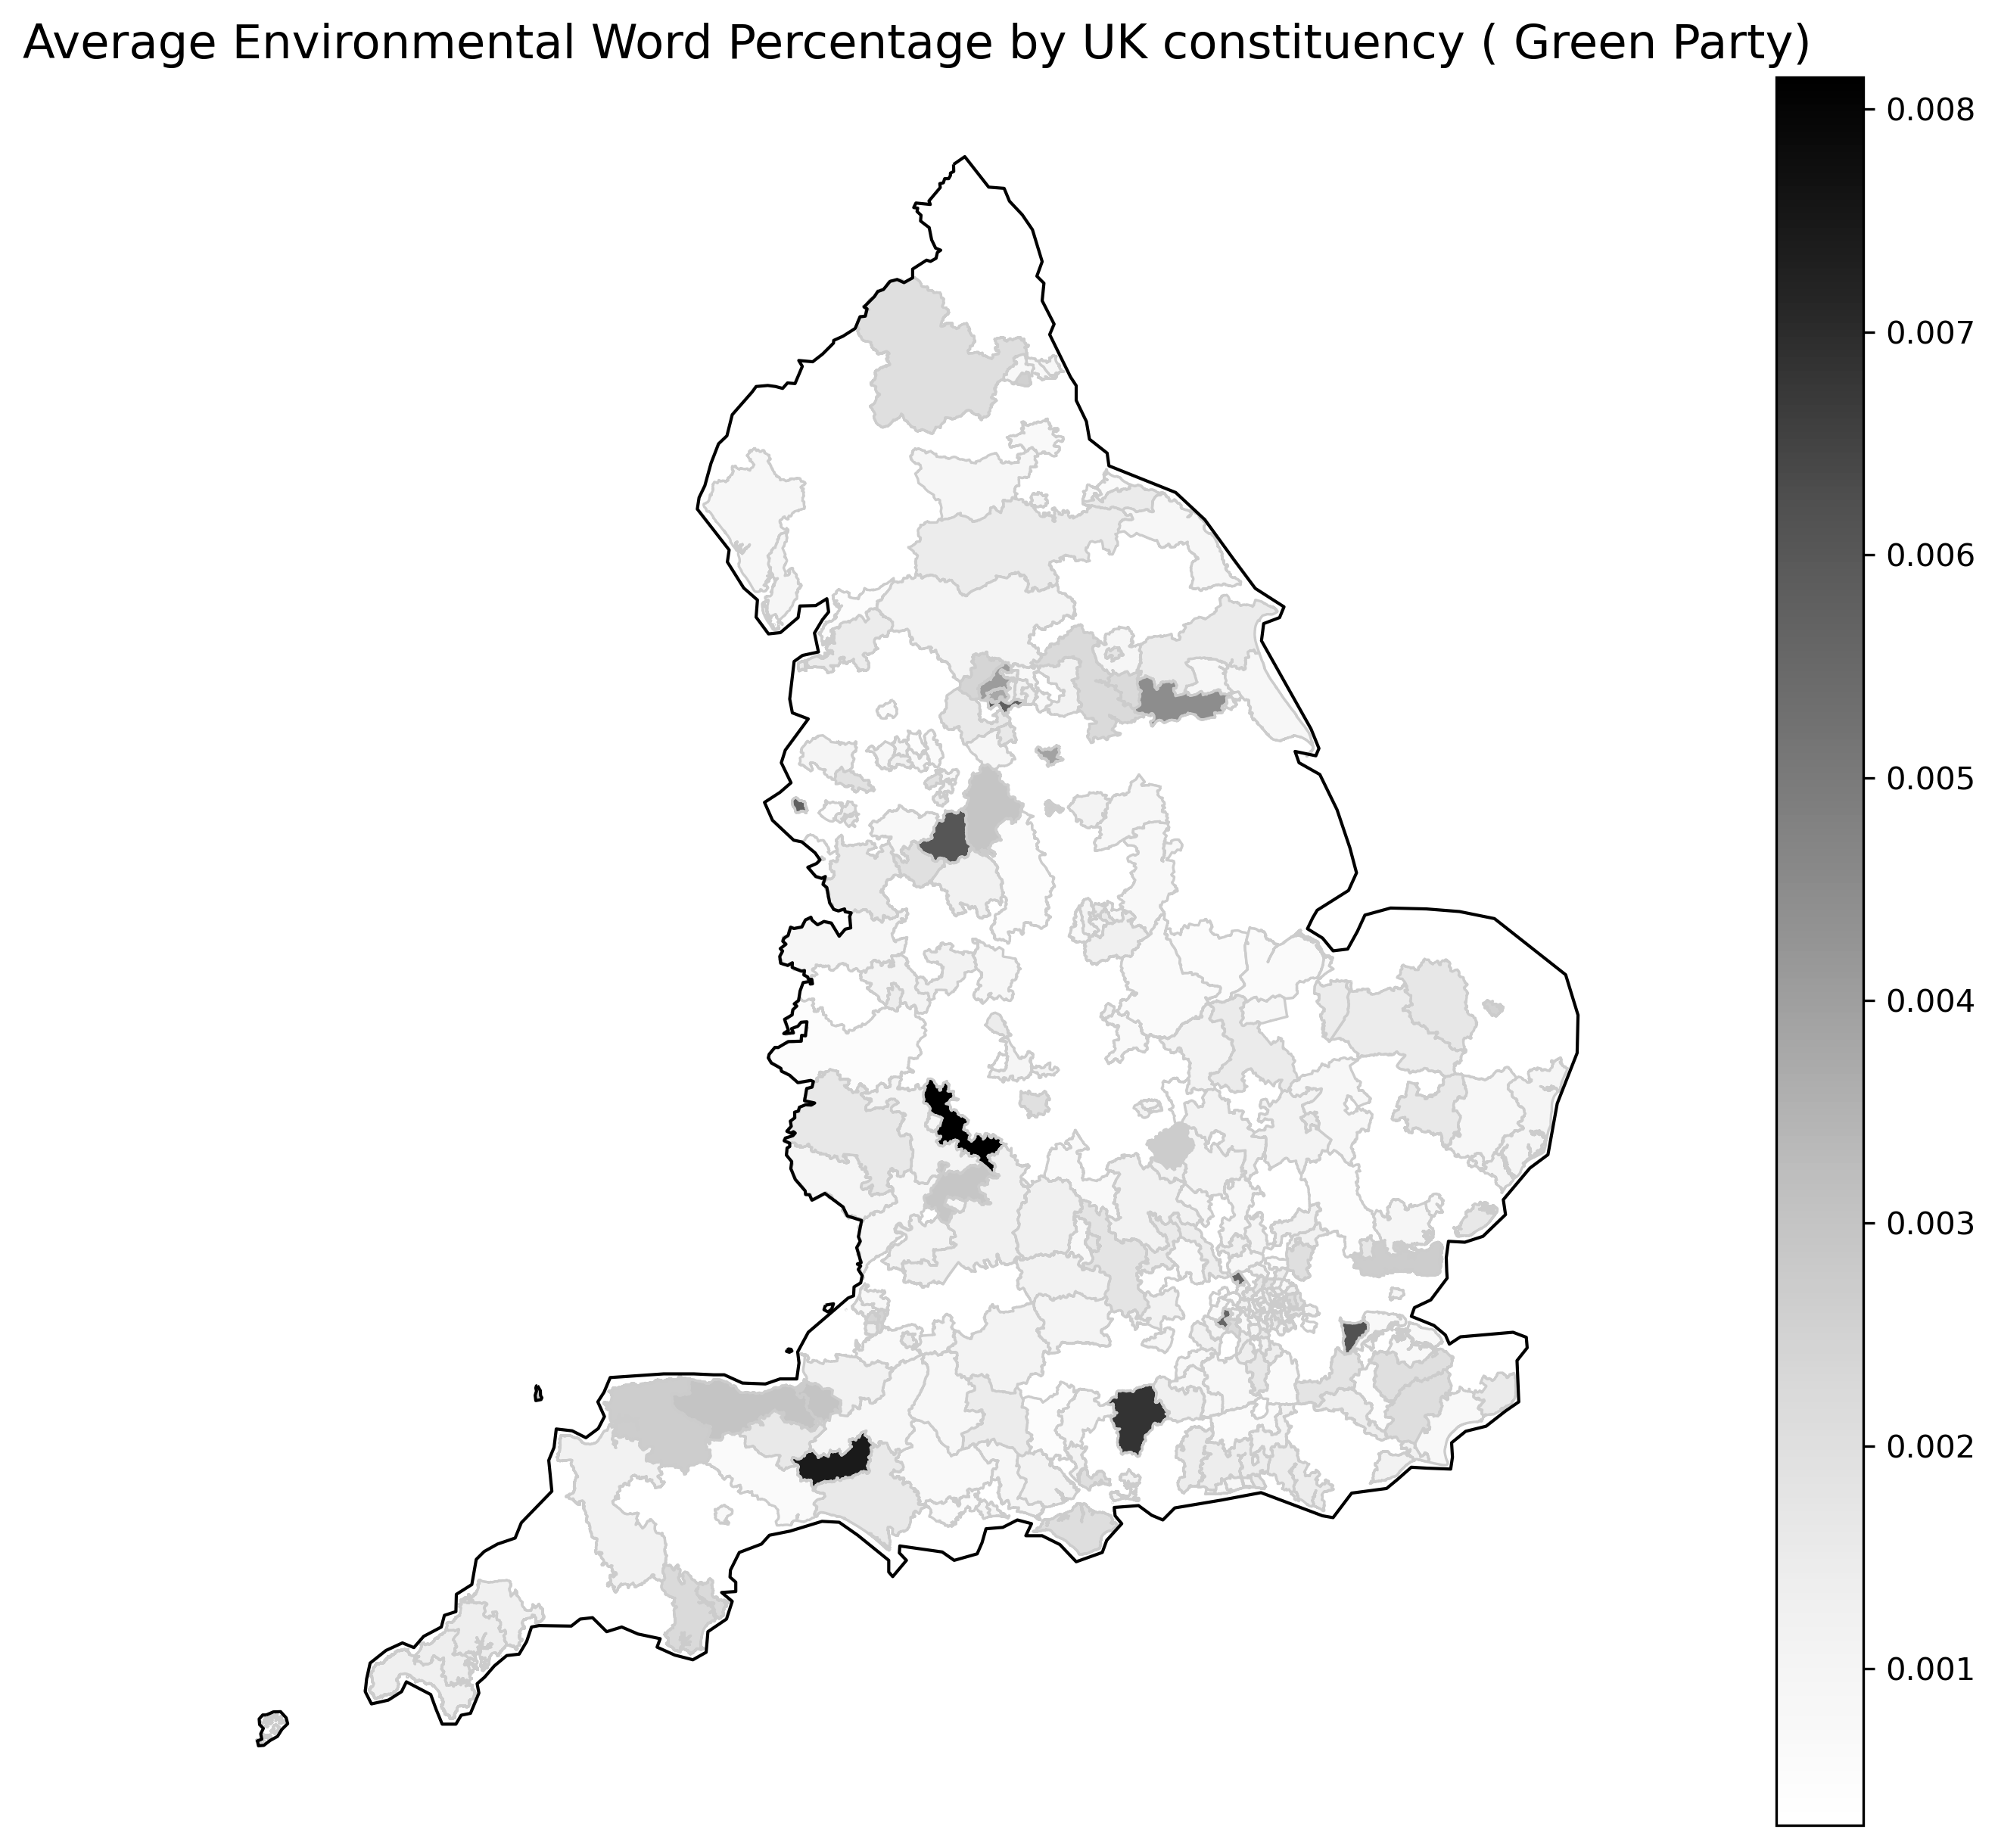
\includegraphics[width=\textwidth,height=0.68\textheight,keepaspectratio]{Appendix_Figure_4.png}
		\caption{Green Party}
	\end{minipage}\hfill
	\begin{minipage}[t]{0.335\textwidth}
		\centering
		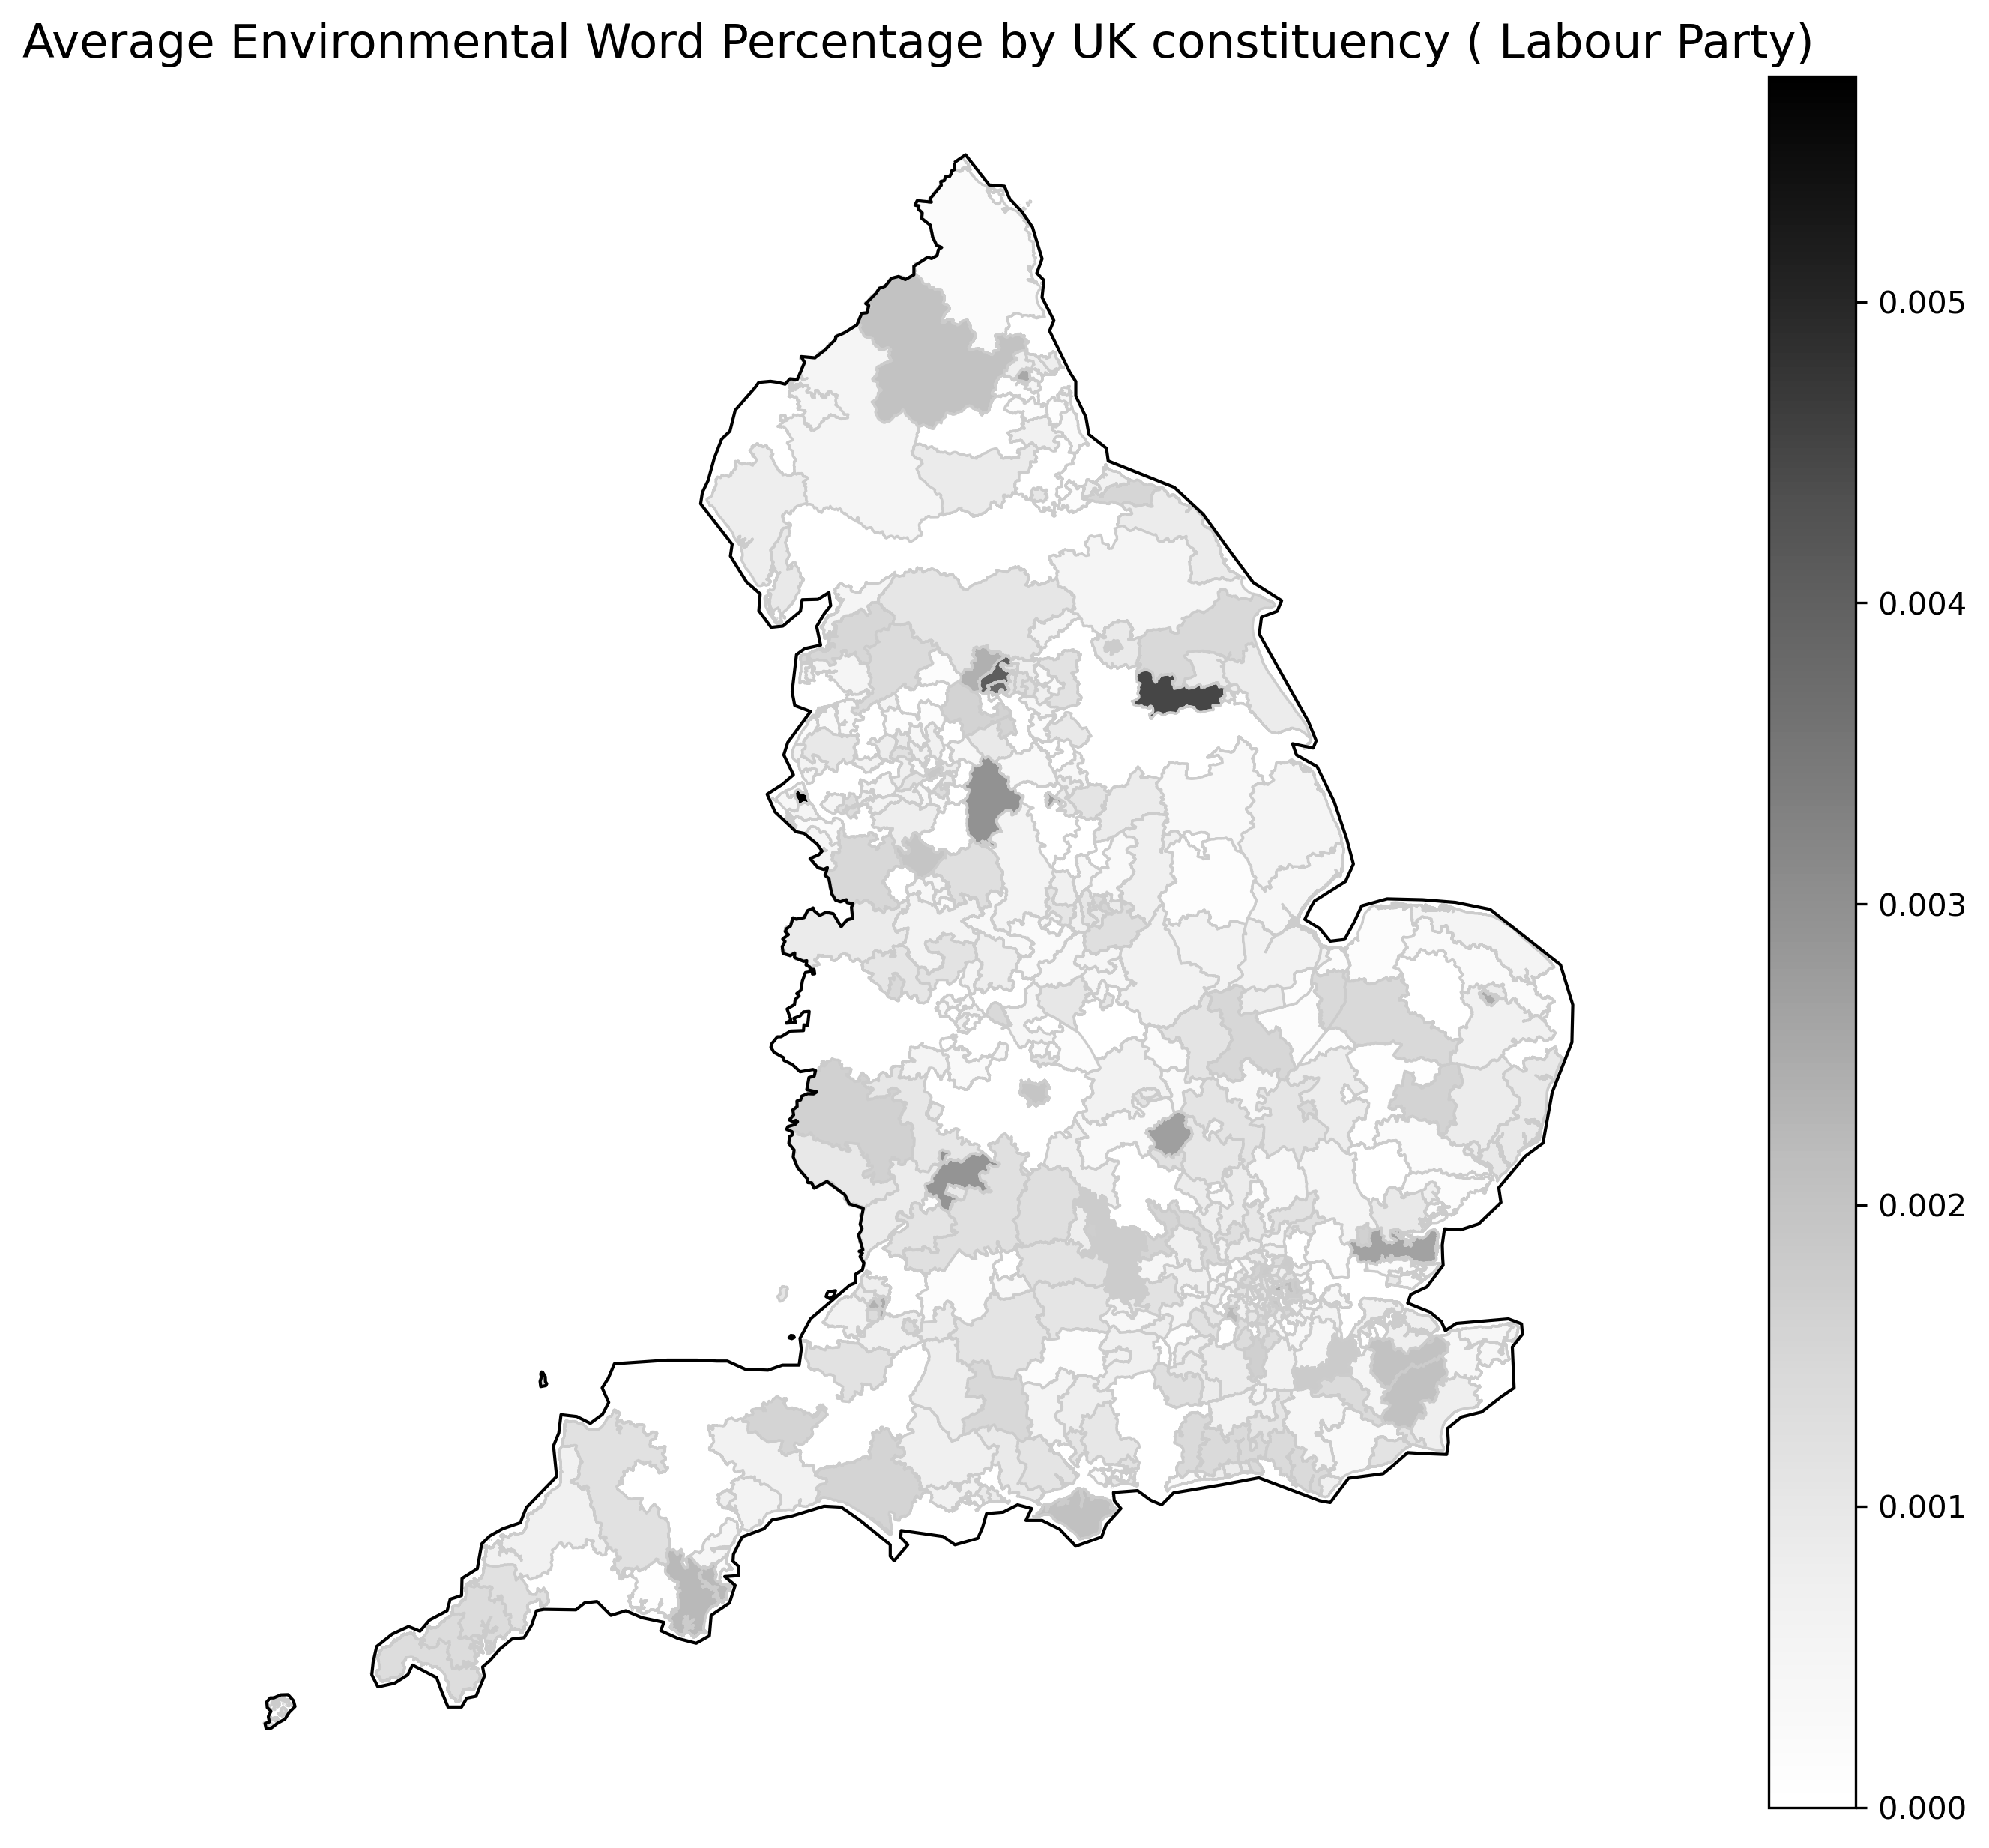
\includegraphics[width=\textwidth,height=0.68\textheight,keepaspectratio]{Appendix_Figure_6.png}
		\caption{Labour Party}
	\end{minipage}
	
	\vspace{0.1cm}  % Adjust space between rows if necessary
	
	% Row 2
	\begin{minipage}[t]{0.335\textwidth}
		\centering
		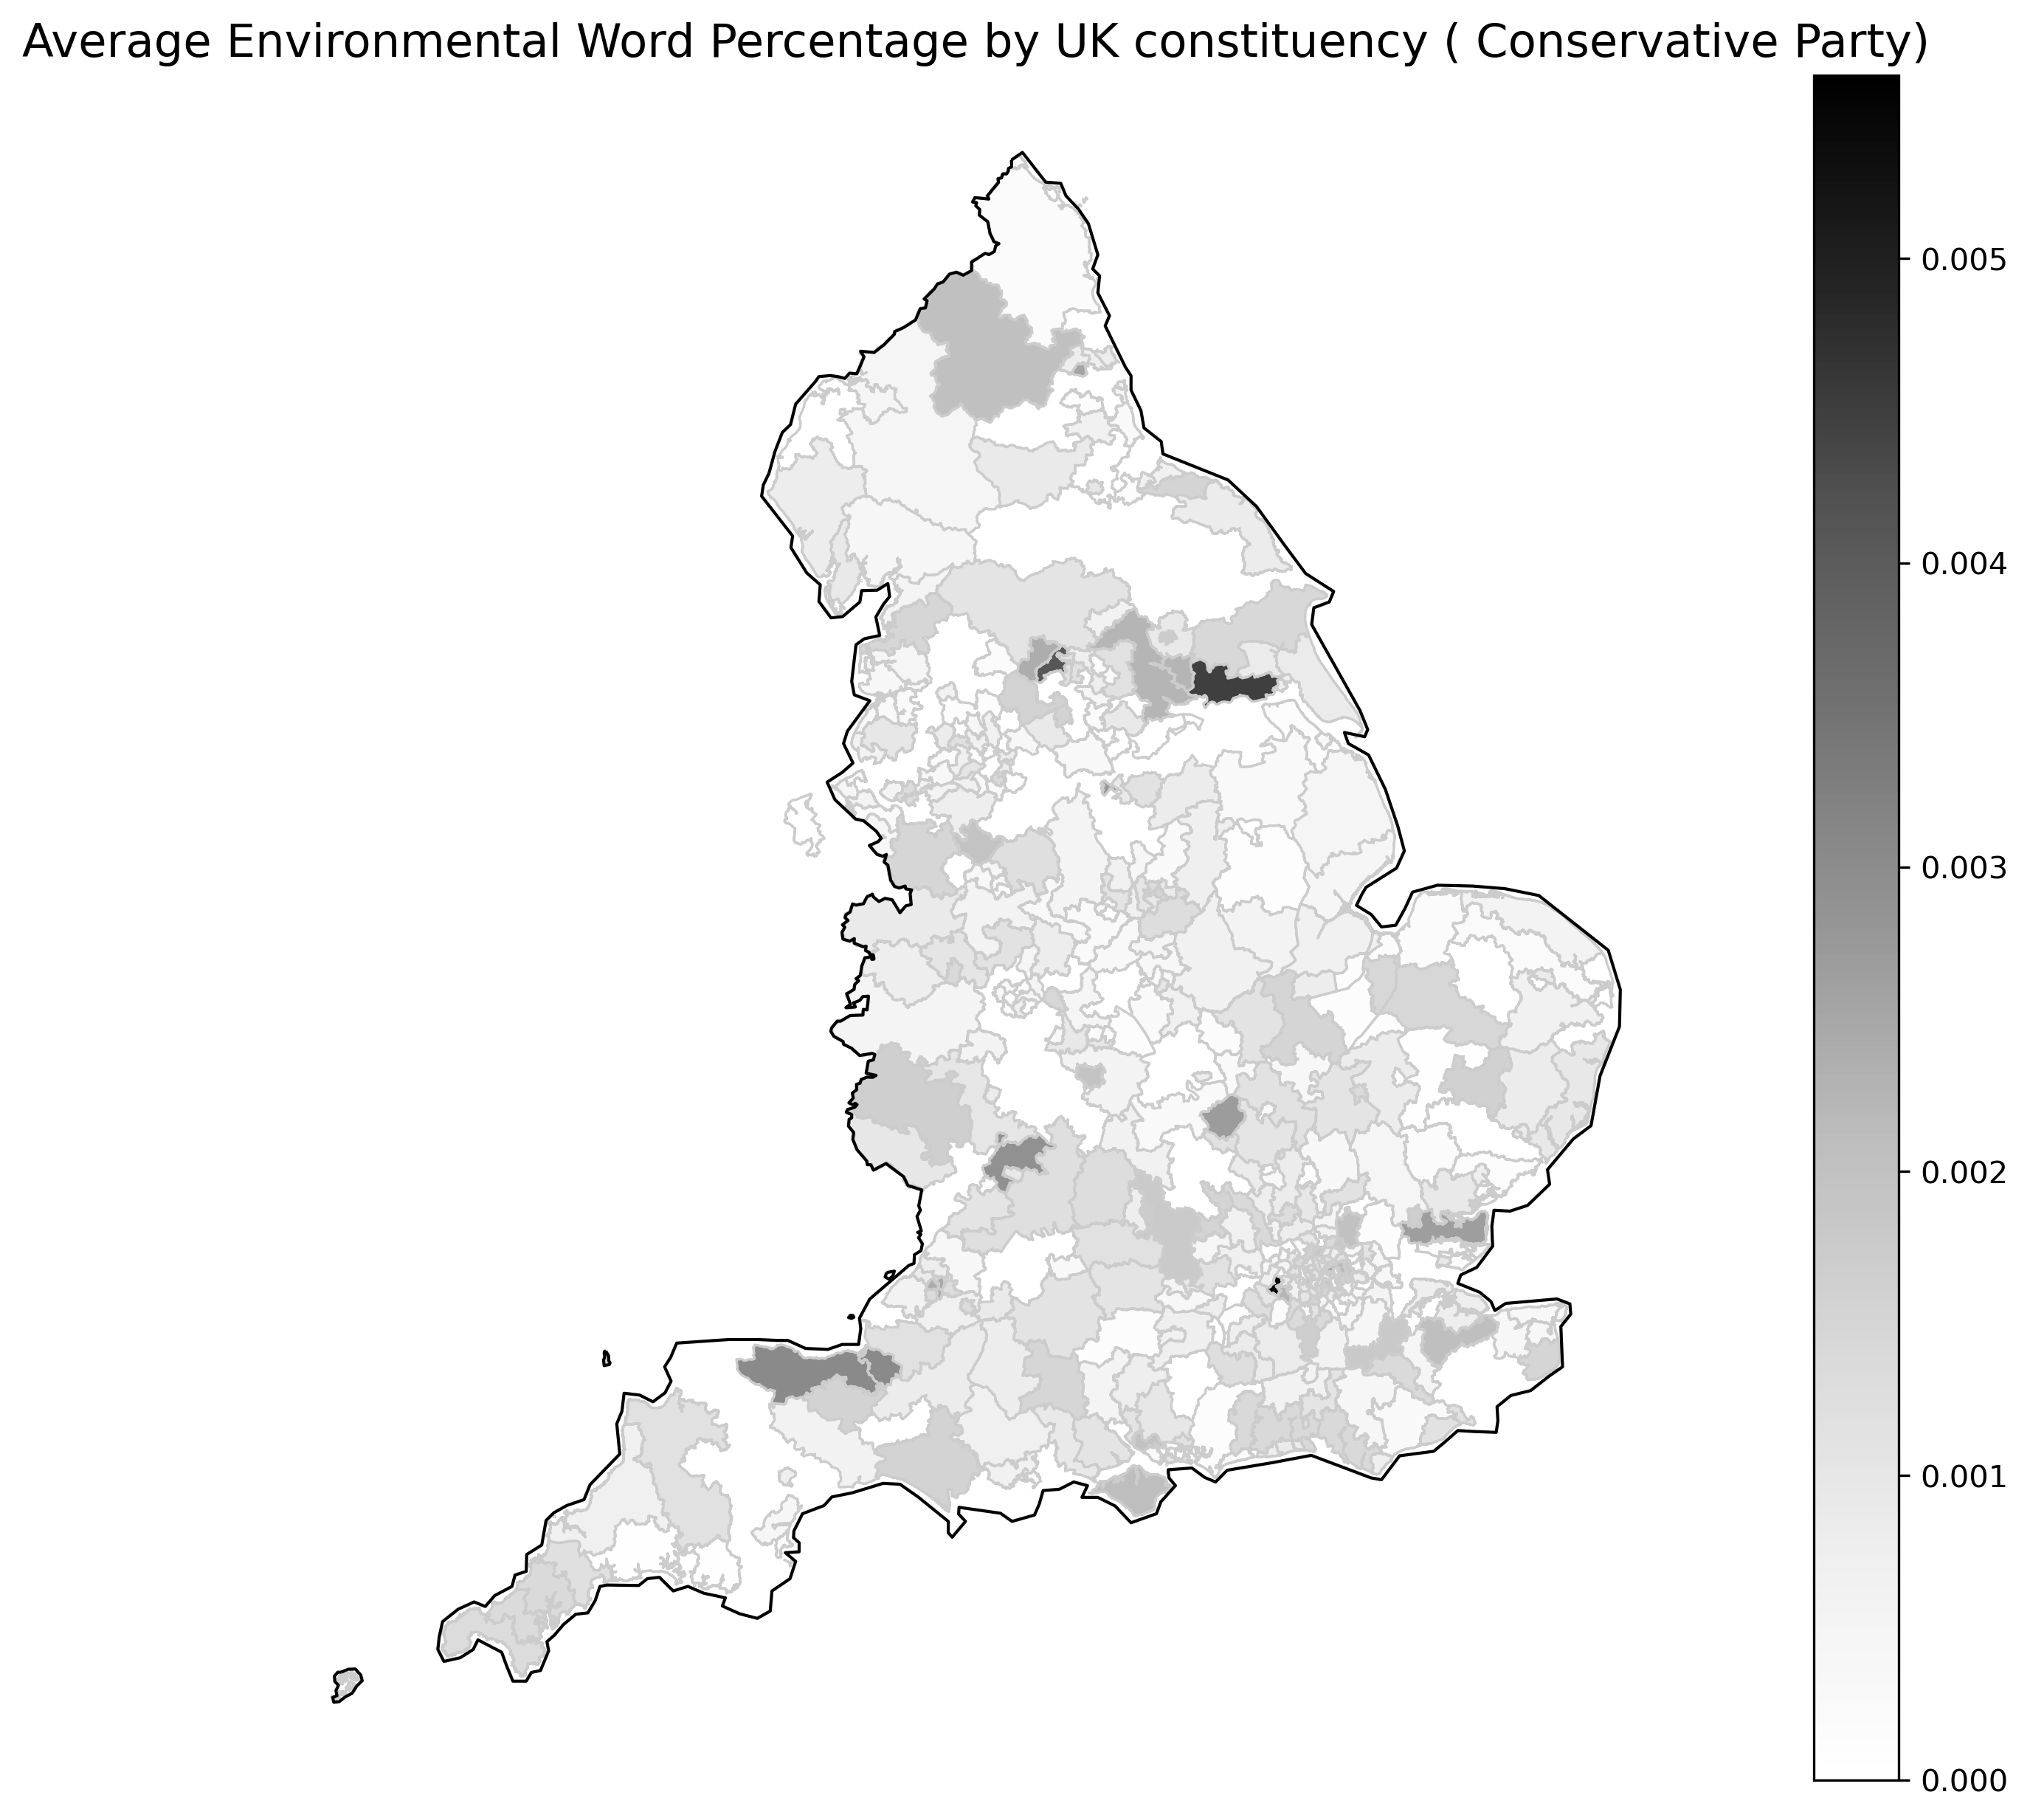
\includegraphics[width=\textwidth,height=0.68\textheight,keepaspectratio]{Appendix_Figure_7.png}
		\caption{Liberal Democrats}
	\end{minipage}\hfill
	\begin{minipage}[t]{0.335\textwidth}
		\centering
		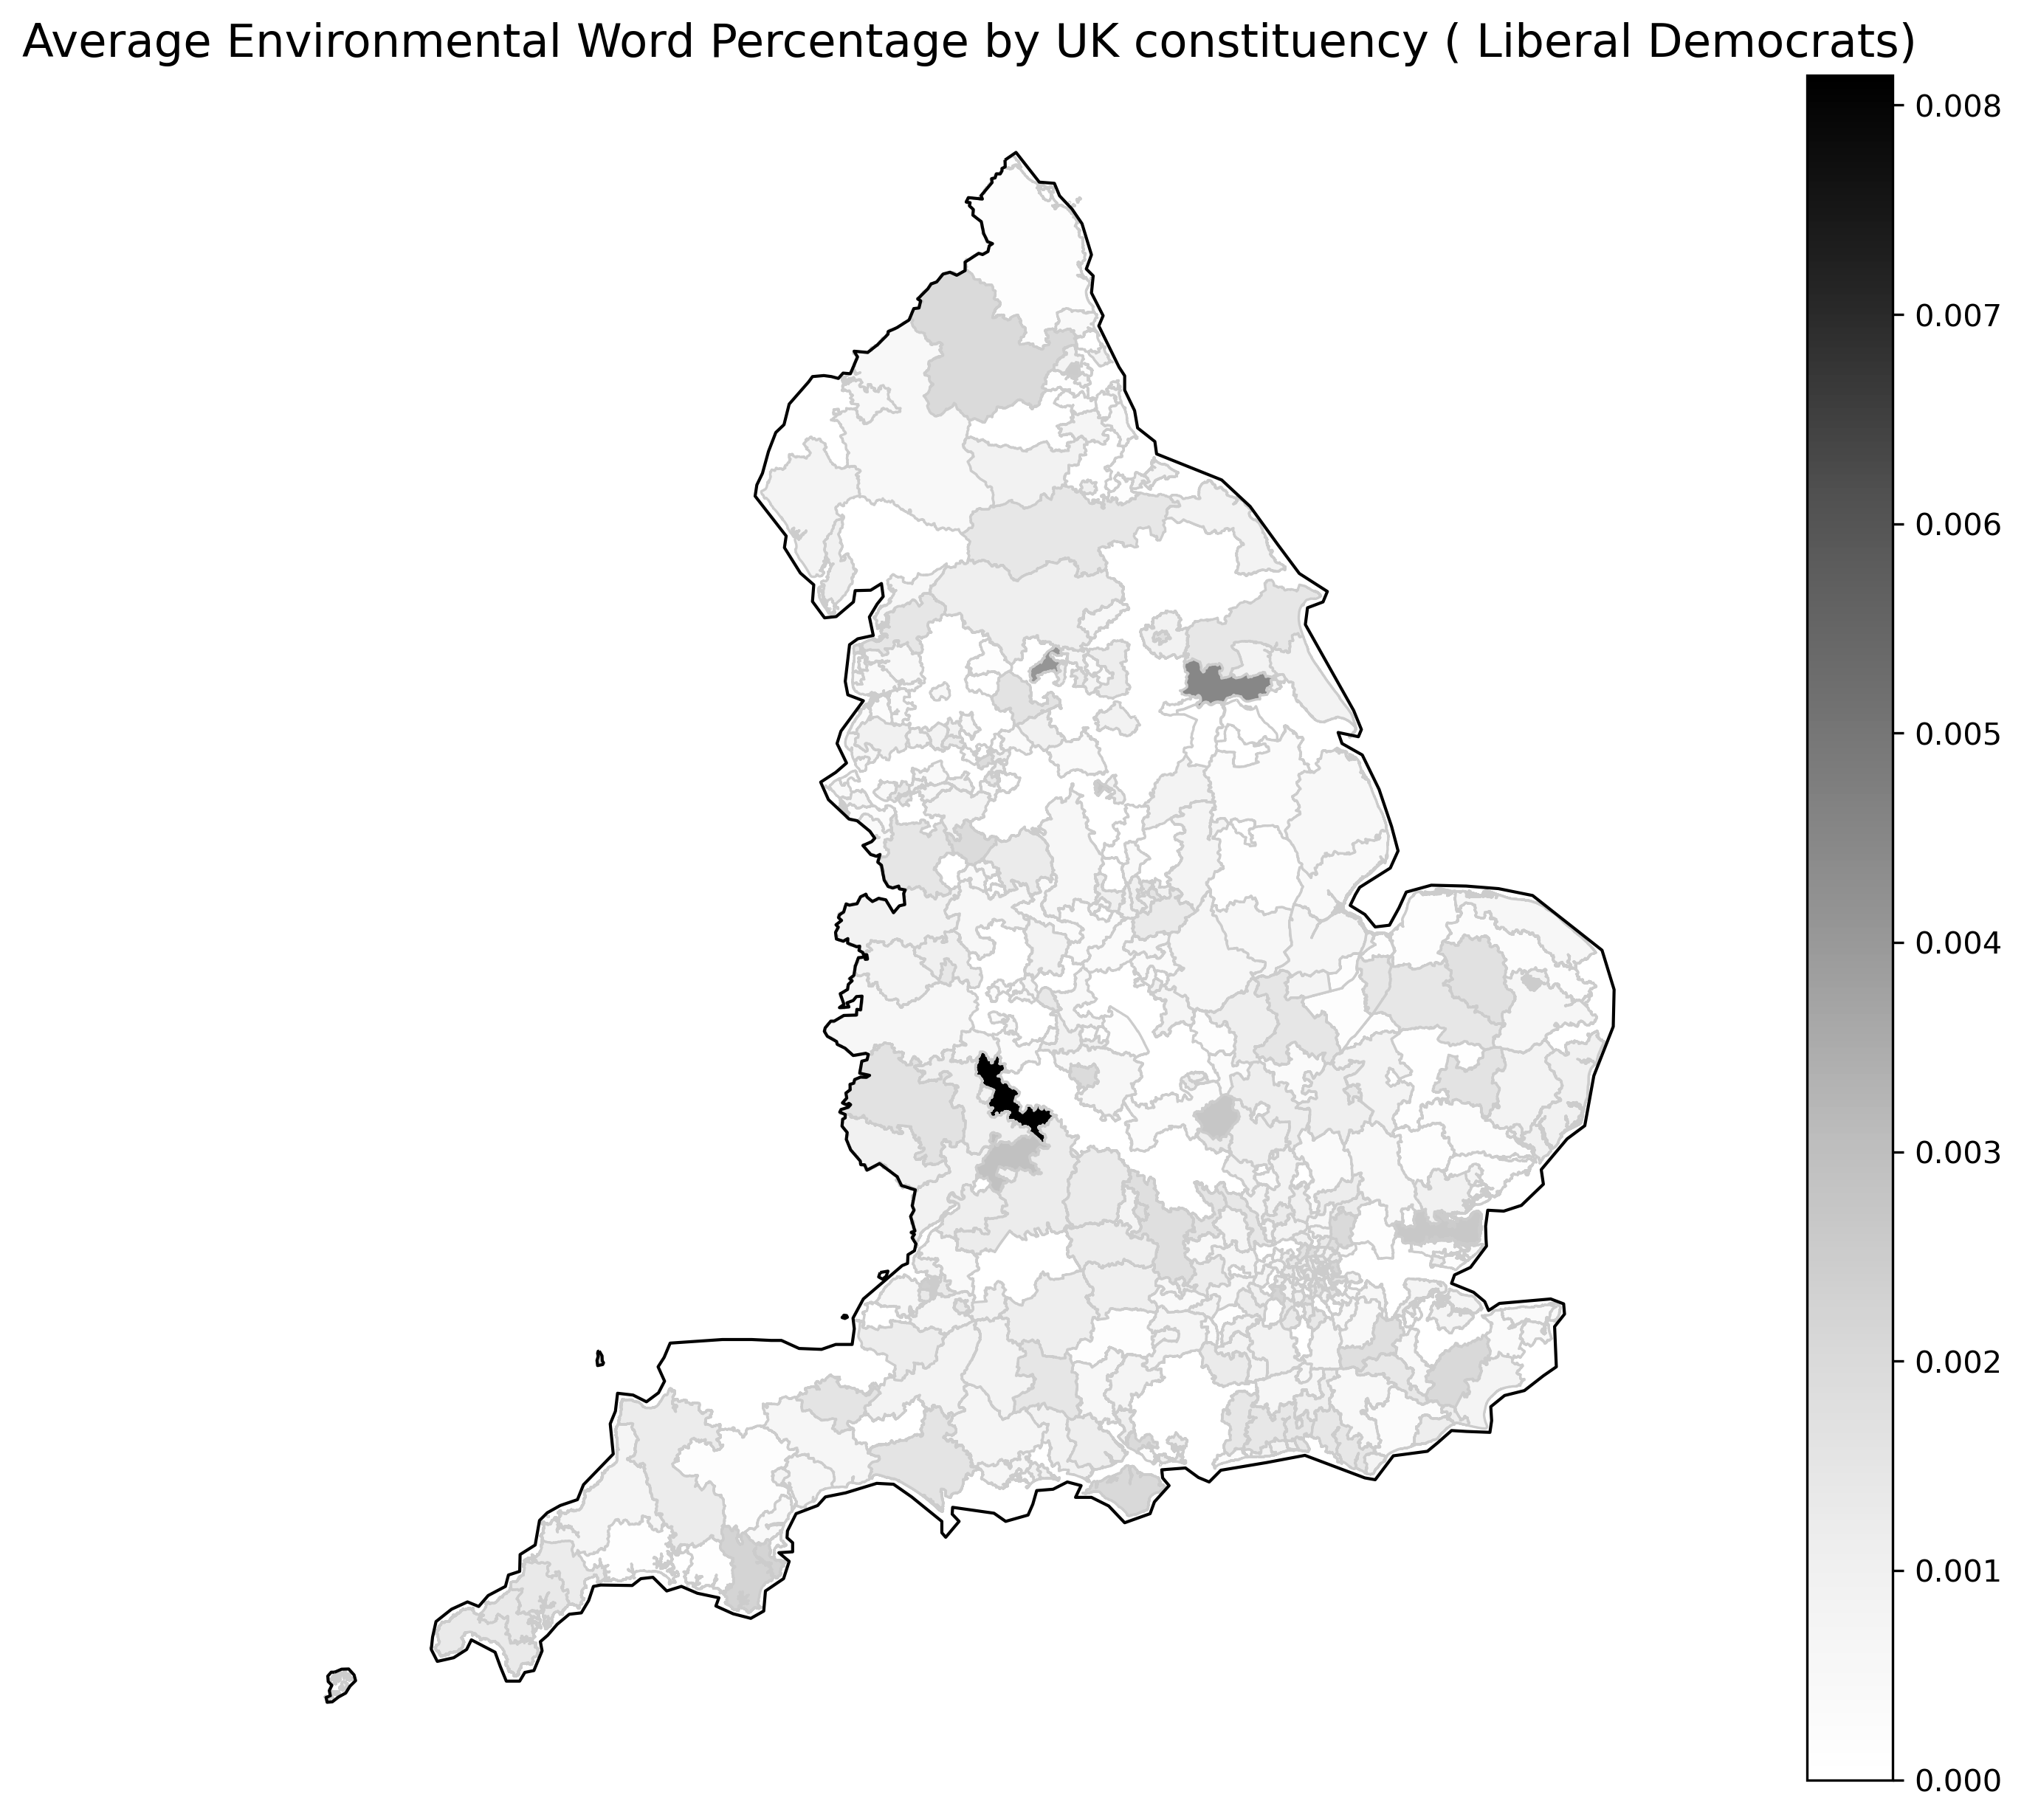
\includegraphics[width=\textwidth,height=0.68\textheight,keepaspectratio]{Appendix_Figure_8.png}
		\caption{UK Independence Party}
	\end{minipage}
	
	\caption{Mean Environmental Mentions by Different Parties Across All Elections}
	\label{fig:parties_environmental_mentions}
\end{figure}



\newpage

\subsection{Breakdown of Number of Leaflets}

\vspace{-0.5cm}


\begin{table}[!htbp] \centering
  \caption{Total Number of Leaflets by Year}
  \label{leaflets_by_year}
\begin{tabular}{@{\extracolsep{5pt}} ccc} 
\\[-1.8ex]\hline
\hline \\[-1.8ex]
 & Election & Total\_Leaflets \\
\hline \\[-1.8ex]
1 &  2010 General Election & 6397 \\
2 &  2015 General Election & 8113 \\
3 &  2017 General Election & 2131 \\
4 &  2019 General Election & 4270 \\
\hline \\[-1.8ex]
\end{tabular}
\end{table}


\begin{table}[!htbp] \centering
  \caption{Number of Leaflets by Party and Year}
  \label{}
\begin{tabular}{@{\extracolsep{5pt}} cccc}
\\[-1.8ex]\hline
\hline \\[-1.8ex]
 & Election & Party & Total\_Leaflets \\ 
\hline \\[-1.8ex]
1 &  2010 General Election &  Conservative Party & 1205 \\
2 &  2010 General Election &  Green Party & 2351 \\ 
3 &  2010 General Election &  Labour Party & 1010 \\
4 &  2010 General Election &  Liberal Democrats & 1694 \\
5 &  2010 General Election &  UK Independence Party & 137 \\
6 &  2015 General Election &  Conservative Party & 884 \\ 
7 &  2015 General Election &  Green Party & 4486 \\
8 &  2015 General Election &  Labour Party & 1012 \\
9 &  2015 General Election &  Liberal Democrats & 1295 \\
10 &  2015 General Election &  UK Independence Party & 436 \\
11 &  2017 General Election &  Conservative Party & 237 \\ 
12 &  2017 General Election &  Green Party & 1196 \\
13 &  2017 General Election &  Labour Party & 411 \\
14 &  2017 General Election &  Liberal Democrats & 245 \\
15 &  2017 General Election &  UK Independence Party & 42 \\
16 &  2019 General Election &  Conservative Party & 439 \\
17 &  2019 General Election &  Green Party & 1552 \\ 
18 &  2019 General Election &  Labour Party & 1145 \\
19 &  2019 General Election &  Liberal Democrats & 1122 \\ 
20 &  2019 General Election &  UK Independence Party & 12 \\
\hline \\[-1.8ex]
\end{tabular}
\end{table}
\newpage

\subsection{Breakdown of Percentage of Political Topics by Year and Party}



\begin{landscape}
\begin{table}[!htbp]
\centering
\caption{Percentage of Leaflet Text by Issue, Party, and Year (Sums to 100\%)}
\label{tab:leaflet-issues}

% Shrink spacing and left-align 'Party' column
\adjustbox{max width=\linewidth}{
\begin{tabular}{@{} c l *{9}{r} @{}}
\toprule
Year & Party & culture & economy & environment & groups & institutions & law\_and\_order & rural & urban & values \\
\midrule

2010 & Conservative      & 0.246 & 54.356 & 3.336 & 0.257 & 28.803 & 5.482 & 1.844 & 0.783 & 4.892 \\
     & Green             & 0.092 & 46.750 & 24.103 & 0.113 & 24.410 & 0.882 & 1.066 & 0.277 & 2.307 \\ 
     & Labour            & 0.445 & 56.489 & 3.080 & 0.375 & 28.197 & 5.151 & 1.226 & 0.543 & 4.493 \\
     & Liberal Democrats & 0.204 & 54.619 & 4.614 & 1.182 & 28.526 & 4.821 & 2.086 & 0.842 & 3.107 \\
     & UK Independence   & 0.217 & 43.232 & 2.967 & 0.477 & 32.727 & 4.722 & 3.877 & 0.477 & 11.306 \\

2015 & Conservative      & 0.277 & 59.409 & 2.574 & 0.262 & 27.263 & 2.679 & 1.753 & 1.121 & 4.662 \\
     & Green             & 0.179 & 47.338 & 22.881 & 0.163 & 22.361 & 0.938 & 1.107 & 0.479 & 4.555 \\
     & Labour            & 0.296 & 64.511 & 2.602 & 0.275 & 24.274 & 2.643 & 1.018 & 0.728 & 3.653 \\
     & Liberal Democrats & 0.329 & 66.786 & 4.171 & 0.892 & 20.866 & 2.074 & 1.031 & 0.776 & 3.076 \\
     & UK Independence   & 1.295 & 53.771 & 2.754 & 0.587 & 25.755 & 4.251 & 4.953 & 0.392 & 6.241 \\

2017 & Conservative      & 0.141 & 50.847 & 1.515 & 0.089 & 36.054 & 1.649 & 1.036 & 0.639 & 8.029 \\
     & Green             & 0.246 & 37.104 & 29.407 & 0.270 & 25.596 & 0.688 & 1.352 & 0.197 & 5.139 \\
     & Labour            & 0.339 & 57.561 & 2.362 & 0.517 & 27.407 & 4.430 & 1.023 & 0.730 & 5.631 \\
     & Liberal Democrats & 0.364 & 53.022 & 2.621 & 0.471 & 34.835 & 2.450 & 1.006 & 0.407 & 4.825 \\
     & UK Independence   & 0.128 & 45.974 & 1.790 & 0.170 & 29.911 & 8.862 & 2.471 & 0.426 & 10.268 \\

2019 & Conservative      & 0.280 & 43.513 & 3.961 & 0.198 & 33.535 & 10.989 & 1.741 & 2.075 & 3.708 \\
     & Green             & 0.126 & 24.589 & 39.261 & 0.101 & 30.913 & 0.506 & 1.720 & 0.632 & 2.150 \\
     & Labour            & 0.460 & 52.440 & 9.752 & 0.503 & 28.277 & 3.407 & 0.979 & 0.588 & 3.594 \\
     & Liberal Democrats & 0.444 & 48.120 & 9.765 & 0.574 & 29.956 & 3.446 & 1.497 & 0.557 & 5.640 \\
     & UK Independence   & 0.000 & 20.395 & 7.895 & 0.658 & 52.632 & 0.658 & 1.974 & 0.000 & 15.789 \\

\bottomrule
\end{tabular}
}
\end{table}
\end{landscape}

\newpage


\subsection{Other Models}


% Table 2: Fixed Effects Model with Election-Year Controls (Time Only)
\begin{table}[!htbp] \centering
	\caption{Fixed Effects Model with Election-Year Controls (Time Only)}
	\label{tab:time_only_fe}
	\footnotesize % Make all text smaller
	\setlength{\tabcolsep}{4pt} % Reduce column spacing
	\renewcommand{\arraystretch}{0.9} % Reduce row spacing
\begin{tabular}{@{\extracolsep{5pt}}lc}
\\[-1.8ex]\hline
\hline \\[-1.8ex]
 & \multicolumn{1}{c}{\textit{Dependent variable:}} \\
 & \multicolumn{1}{c}{\textit{Environmental Mention Percentage}} \\
\cline{2-2}
\\[-1.8ex] & \textasciitilde . \\
\hline \\[-1.8ex]
 Party Conservative Party & $-$0.005$^{***}$ \\
	& (0.0001) \\
 Party Labour Party & $-$0.005$^{***}$ \\
	& (0.0001) \\
 Party Liberal Democrats & $-$0.005$^{***}$ \\
	& (0.0001) \\
 Party UK Independence Party & $-$0.005$^{***}$ \\
	& (0.0001) \\
 Median Age & $-$0.00001 \\
	& (0.00001) \\ 
 Rural Proportion & 0.0001 \\
	& (0.0002) \\
 Working Class Proportion & 0.004$^{*}$ \\
	& (0.002) \\
 Intermediate Proportion & 0.003 \\
	& (0.002) \\
 Professional Proportion & 0.003$^{*}$ \\
	& (0.002) \\
 Total Student Percentage & 0.003 \\
	& (0.002) \\
 Overall Weather Standard Deviation & 0.00001 \\
	& (0.00001) \\
 Liberal Democrat Share & 0.0004 \\ 
	& (0.0005) \\
 Labour Party Share & 0.0004 \\
	& (0.0005) \\
 Other Party Share & 0.0004 \\
	& (0.0005) \\
 Conservative Party Share & 0.0004 \\
	& (0.0005) \\
 \hline \\[-1.8ex]
Observations & 3,904 \\
R$^{2}$ & 0.569 \\
Adjusted R$^{2}$ & 0.168 \\
Residual Std. Error & 0.001 (df = 3885) \\
F Statistic & 359.861$^{***}$ (df = 18; 3885) \\
\hline
\hline \\[-1.8ex]
\textit{Note:}  & \multicolumn{1}{r}{$^{*}$p$<$0.1; $^{**}$p$<$0.05; $^{***}$p$<$0.01} \\ 
\end{tabular}
\end{table}

% Table 3: Fixed Effects Model with Election-Year Controls (Time and Constituency)
\begin{table}[!htbp] \centering
	\caption{Fixed Effects Model with Election-Year Controls (Time and Constituency)}
	\label{tab:time_constituency_fe}
	\footnotesize % Make all text smaller
	\setlength{\tabcolsep}{4pt} % Reduce column spacing
	\renewcommand{\arraystretch}{0.9} % Reduce row spacing
\begin{tabular}{@{\extracolsep{5pt}}lc}
\\[-1.8ex]\hline
\hline \\[-1.8ex]
 & \multicolumn{1}{c}{\textit{Dependent variable:}} \\
 & \multicolumn{1}{c}{\textit{Environmental Mention Percentage}} \\
\cline{2-2}
\\[-1.8ex] & \textasciitilde . \\
\hline \\[-1.8ex]
 Party Conservative Party & $-$0.005$^{***}$ \\
	& (0.0001) \\
 Party Labour Party & $-$0.005$^{***}$ \\
	& (0.0001) \\
 Party Liberal Democrats & $-$0.004$^{***}$ \\
	& (0.0001) \\
 Party UK Independence Party & $-$0.005$^{***}$ \\
	& (0.0001) \\
 \hline \\[-1.8ex] 
Observations & 5,417 \\
R$^{2}$ & 0.660 \\
Adjusted R$^{2}$ & 0.627 \\
Residual Std. Error & 0.001 (df = 5400) \\
F Statistic & 359.861$^{***}$ (df = 4; 5400) \\
\hline
\hline \\[-1.8ex]
\textit{Note:}  & \multicolumn{1}{r}{$^{*}$p$<$0.1; $^{**}$p$<$0.05; $^{***}$p$<$0.01} \\
\end{tabular}
\end{table}




\end{document}
